\documentclass[letterpaper,12pt,notitlepage,twoside]{report}

%\newcommand{\watermark}{Deep Learning}
\newcommand{\booktopic}{Deep Learning}
\newcommand{\lastname}{Okoli}
\usepackage{NoteStyle}
\usepackage{placeins}
\usepackage{listings}% http://ctan.org/pkg/listings
\lstset{
  basicstyle=\ttfamily,
  mathescape
}
\usepackage{pifont} % to use the ding itemize
\usepackage[dvipsnames]{xcolor}


\definecolor{codegreen}{rgb}{0,0.6,0}
\definecolor{codegray}{rgb}{0.5,0.5,0.5}
\definecolor{codepurple}{rgb}{0.58,0,0.82}
\definecolor{backcolour}{rgb}{0.95,0.95,0.92}

\lstdefinestyle{mystyle}{
    backgroundcolor=\color{backcolour},   
    commentstyle=\color{codegreen},
    keywordstyle=\color{magenta},
    numberstyle=\tiny\color{codegray},
    stringstyle=\color{codepurple},
    basicstyle=\ttfamily\footnotesize,
    breakatwhitespace=false,         
    breaklines=true,                 
    captionpos=b,                    
    keepspaces=true,                 
    numbers=left,                    
    numbersep=5pt,                  
    showspaces=false,                
    showstringspaces=false,
    showtabs=false,                  
    tabsize=2
}

\lstset{style=mystyle}

\title{Deep Learning}
\author{Chuks Okoli}
\date{\footnotesize Last Updated: \today}

\hypersetup{
  pdftitle={Deep Learning},
  pdfauthor={Chuks Okoli},
  pdfsubject={},
}


% ToC on the title page:
% https://tex.stackexchange.com/a/45863
\makeatletter
\newcommand*{\toccontents}{\@starttoc{toc}}
\makeatother

\begin{document}

\begin{titlepage}
  \pagestyle{plain}
  \maketitle
  \setcounter{tocdepth}{2}

  \pdfbookmark[section]{\contentsname}{toc}
  \toccontents
  % Separate page:
  % \tableofcontents
\end{titlepage}

% ---------------- Chapter 1. Welcome to Deep learning ----------------------%
\chapter{Welcome to Deep Learning} \label{ch:1}
\inspiration{Just as electricity transformed almost everything 100 years ago, today I actually have a hard time thinking of an industry that I don’t think AI (Artificial Intelligence) will transform in the next several years.}{Andrew Ng}{DeepLearning.AI}

\firstletter{Hello there}, and welcome to \booktopic. This work is a culmination of hours of effort to create my reference for deep learning. All the explanations are in my own words but majority of the contents are based on DeepLearning.AI's specialization in \href{https://www.deeplearning.ai/courses/deep-learning-specialization/}{Deep Learning}.


% ------------------ Introduction to Deep learning -----------------------------%
\section{Introduction to Deep learning}
The term, Deep Learning, refers to training Neural Networks, sometimes very large Neural Networks.  In order to predict the price of a house based on its size for example, we can apply linear regression as a method for fitting a function to predict house prices. An alternative approach would be to use a simple neural network to model the relationship between house size and price. 

The simple neural network consists of a single neurons, which takes an input (e.g., house size) and outputs a prediction (e.g., house price). The neuron computes a linear function of the input and applies a rectified linear unit (ReLU) activation function to ensure non-negativity. Each neuron in the network computes a function of the input features and contributes to the overall prediction. When extended to multiple features, each feature is represented by a separate neuron, and the network learns to predict the house price based on these features.

Neural networks are useful in supervised learning scenarios, where the goal is to map input features to corresponding output labels. Given enough training data, neural networks can learn complex mappings from inputs to outputs.

\begin{figure}[h]
	\centering
	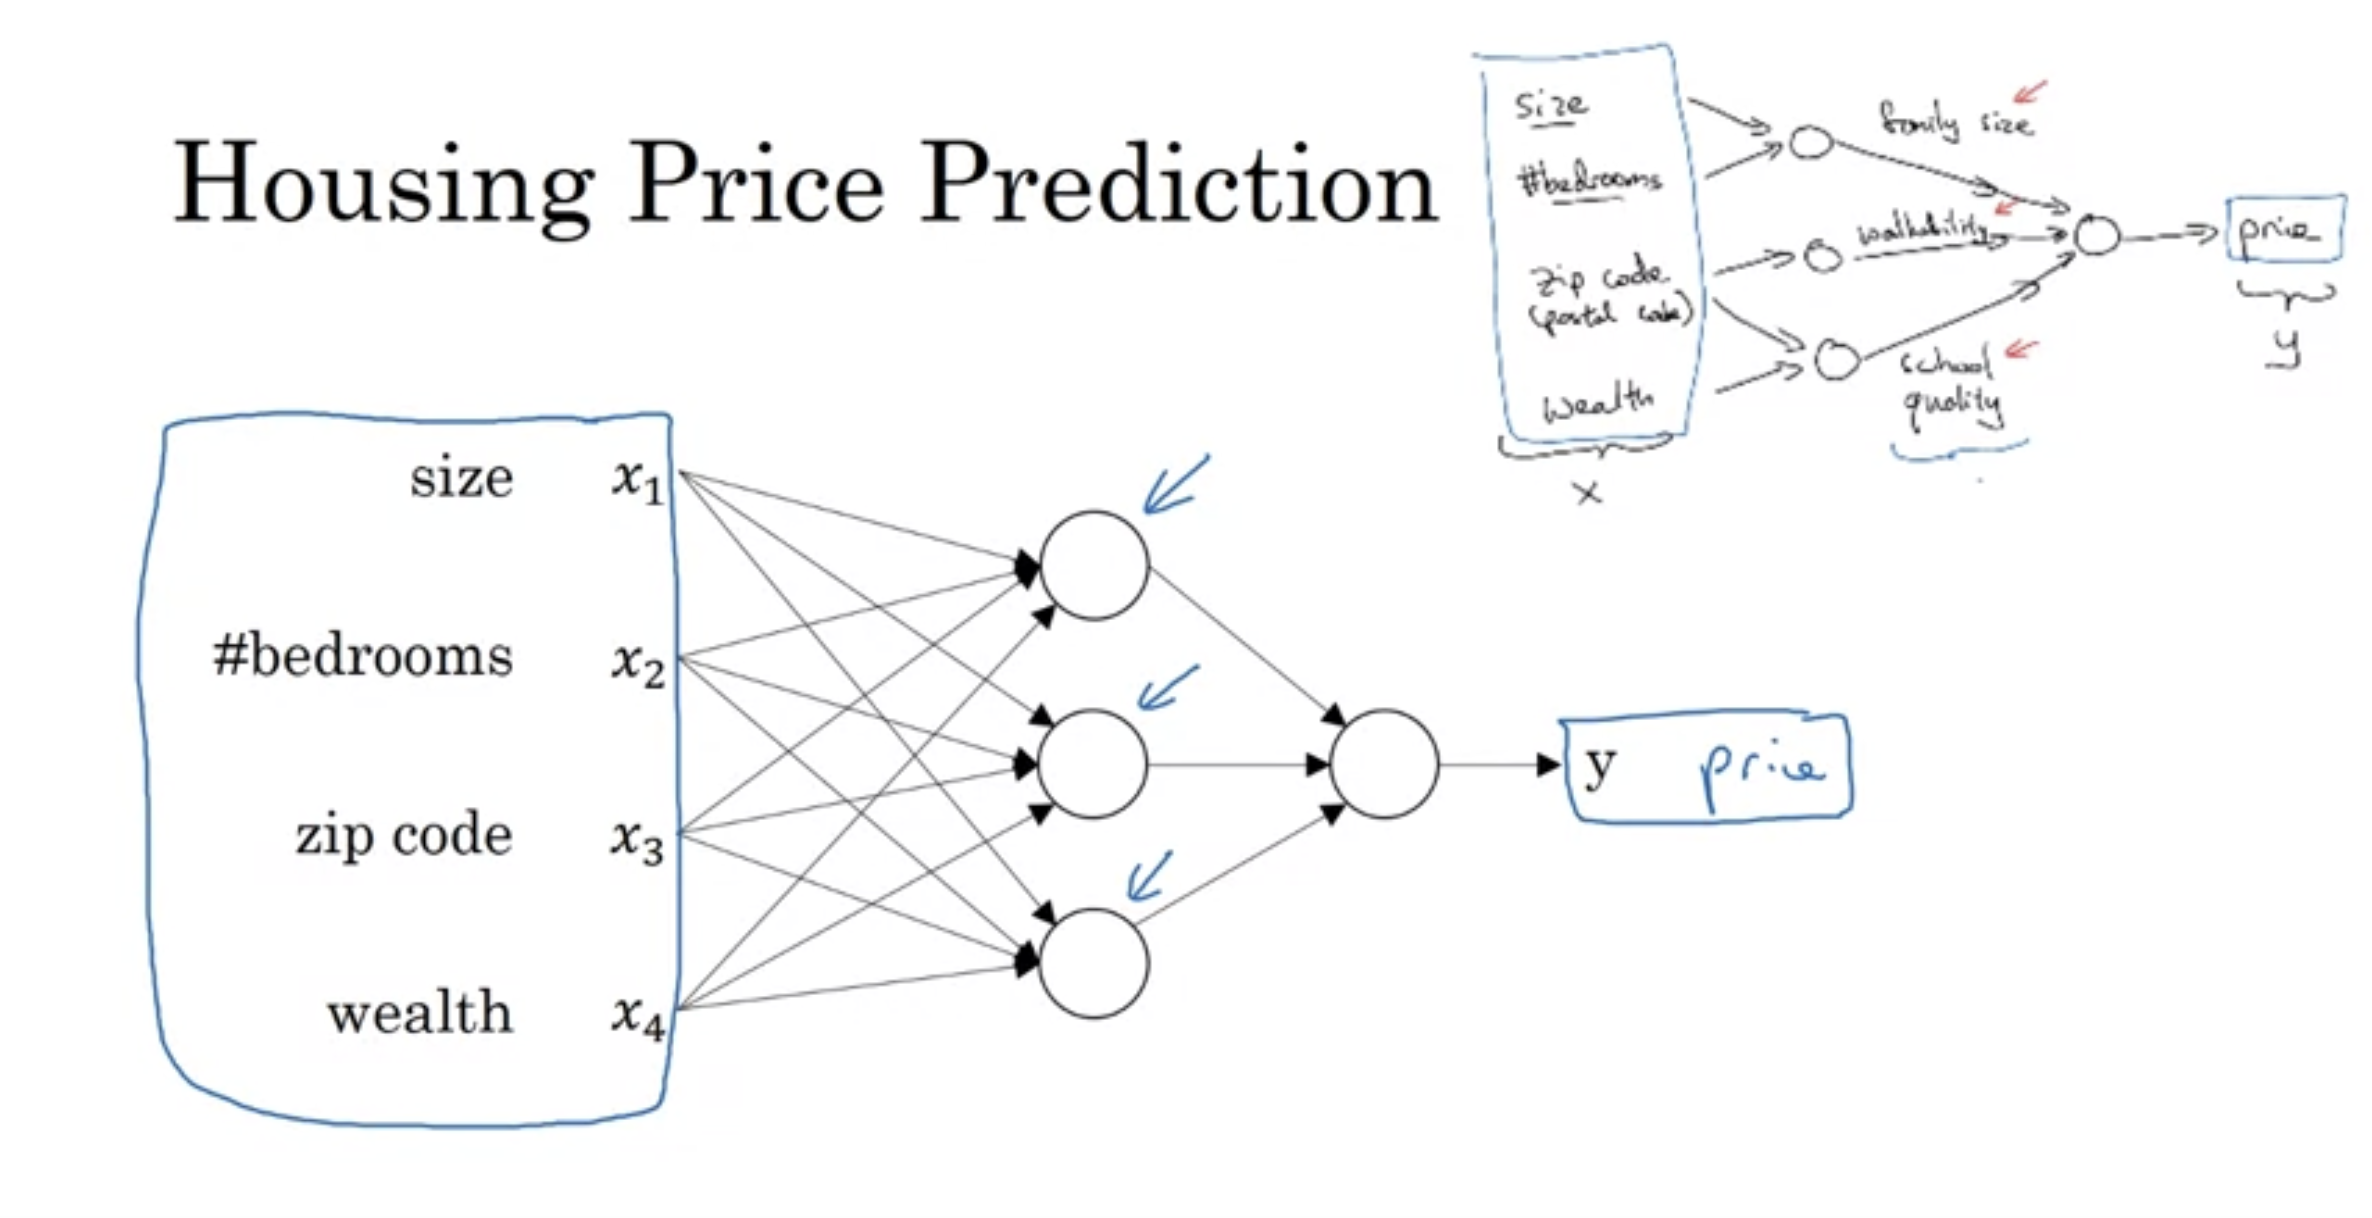
\includegraphics[width=0.75\textwidth]{Images/Simple Neural Network.png}
	\caption{A Simple Neural Network for House Price Prediction}
	\label{fig:1}
\end{figure}
\FloatBarrier

\subsection{Supervised Learning with Neural Networks}
Neural networks have gained a lot of attention lately for their ability to solve complex problems effectively. In supervised learning, you input data and aim to predict an output. Examples include predicting house prices or online ad clicks. Neural networks have been successful in various applications, like online advertising, computer vision, speech recognition, and machine translation. Different types of neural networks are used based on the nature of the data, such as convolutional neural networks for images and recurrent neural networks for sequential data. Structured data, like database entries, and unstructured data, like images or text, are both now interpretable by neural networks, thanks to recent advancements. While neural networks are often associated with recognizing images or text, they also excel in processing structured data, leading to improved advertising and recommendation systems. The techniques covered in this course apply to both structured and unstructured data, reflecting the versatility of neural networks in various applications.

\begin{figure}[h]
	\centering
	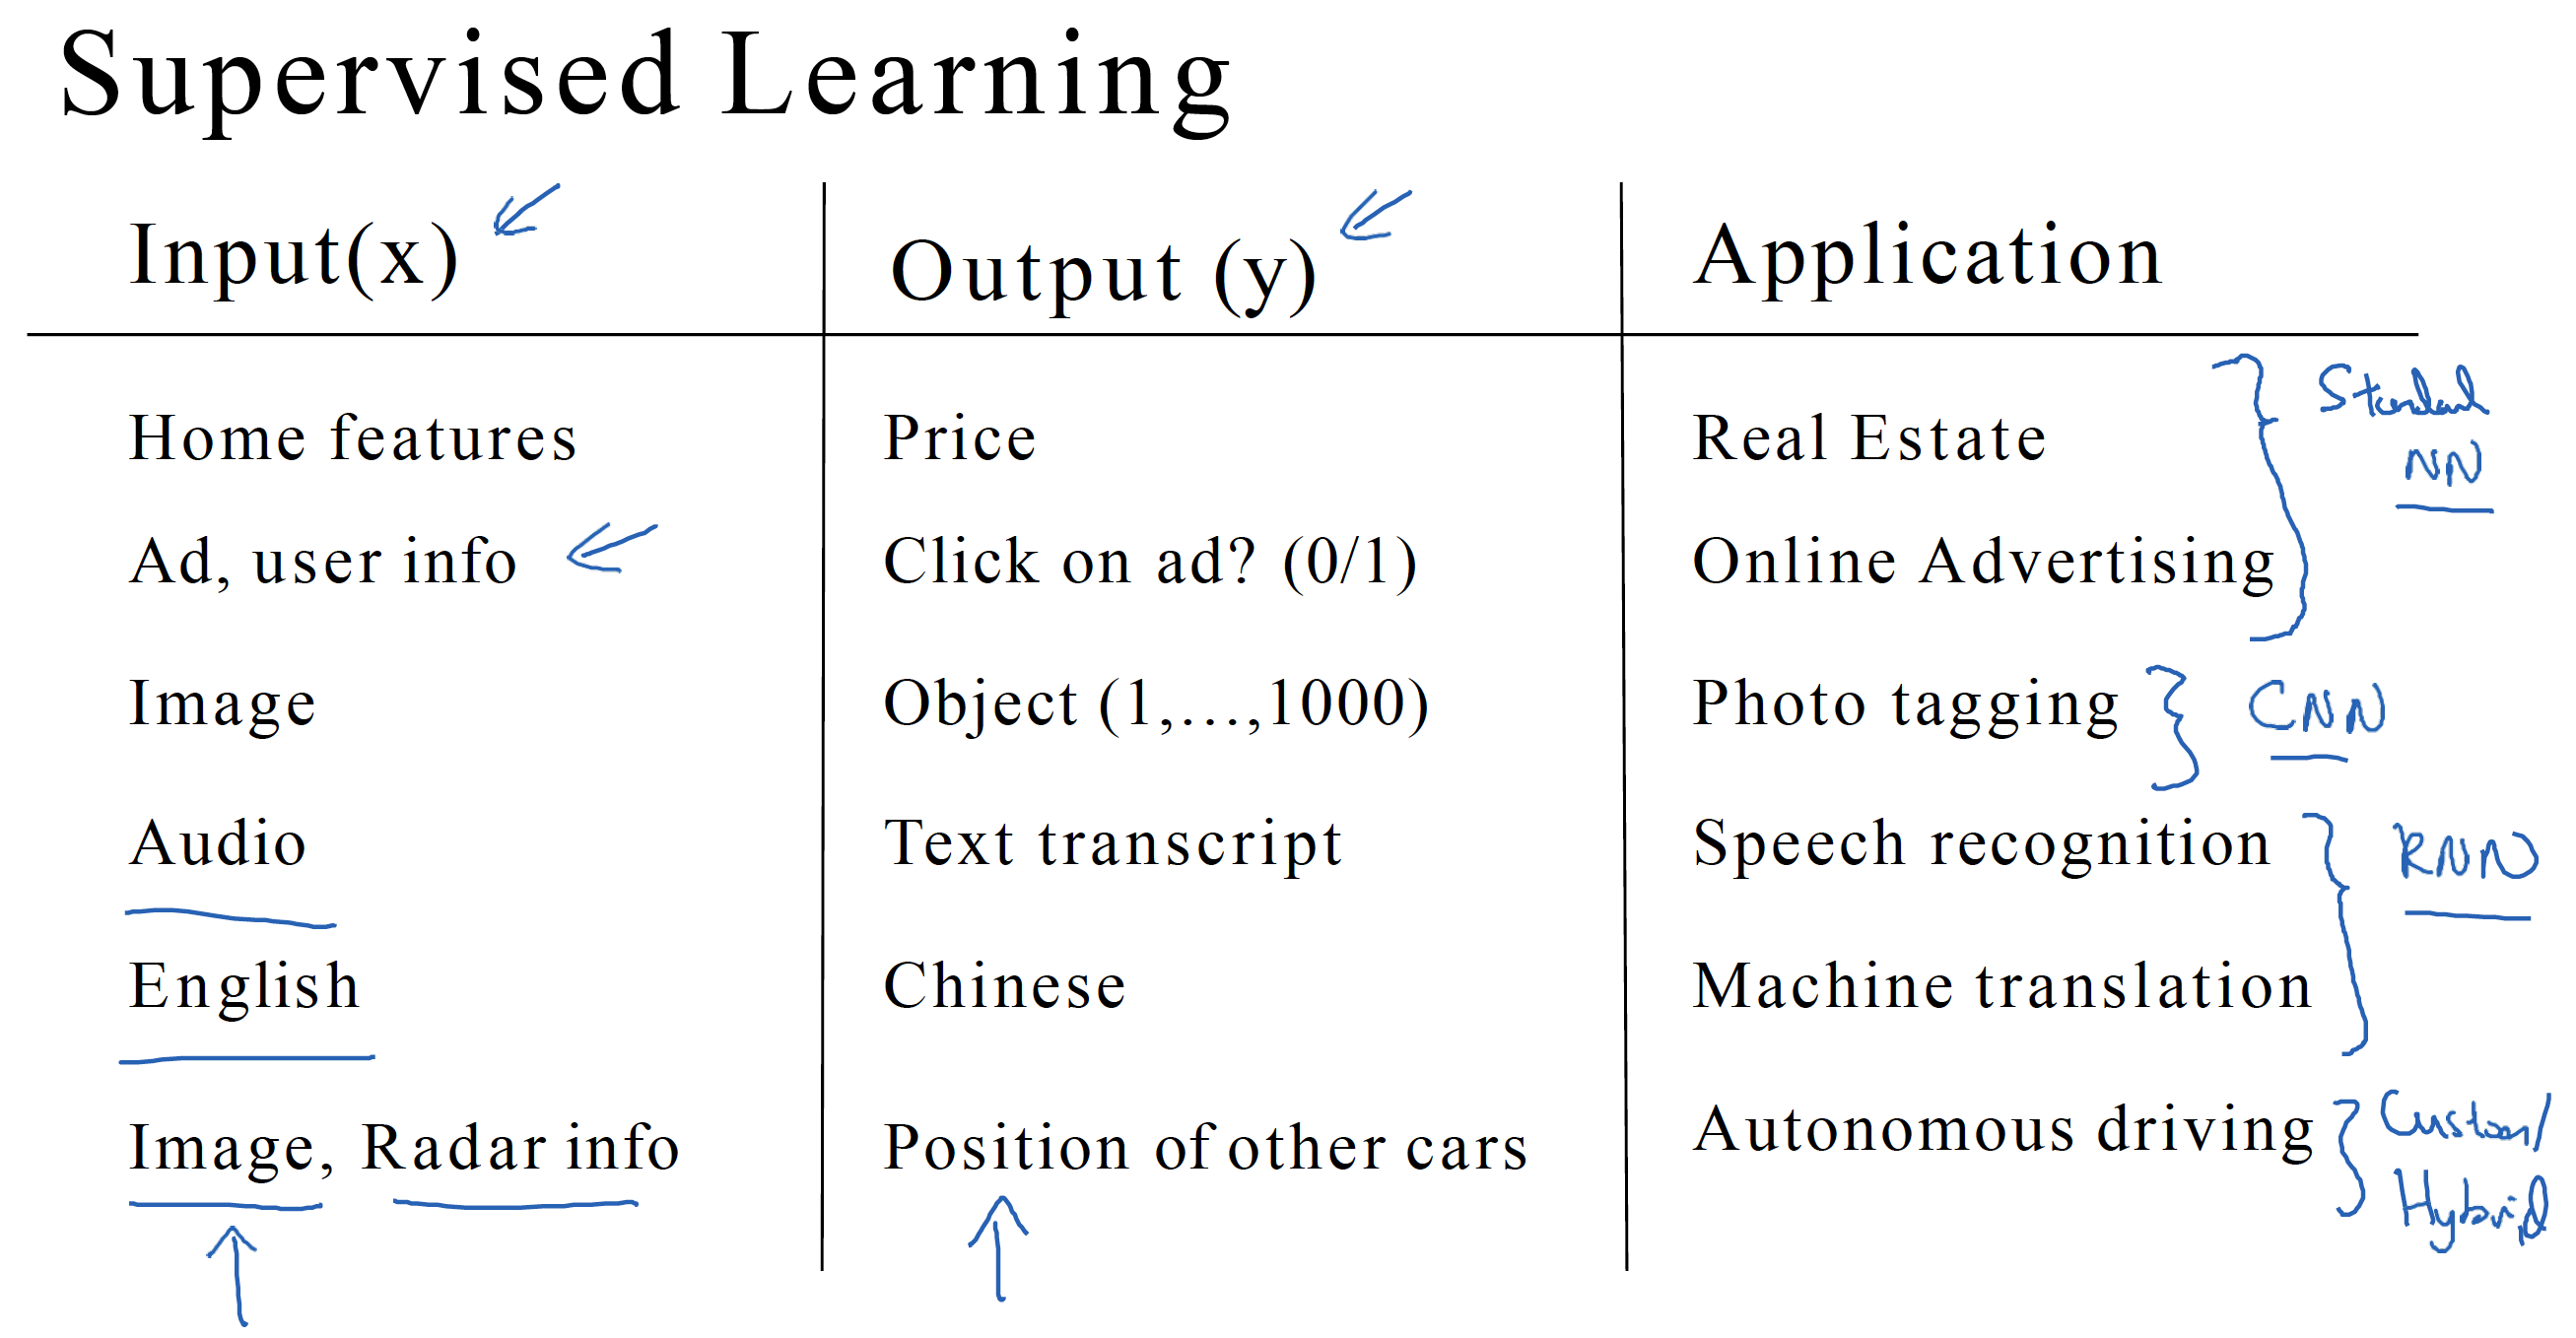
\includegraphics[width=0.75\textwidth]{Images/Supervised learning.png}
	\caption{Examples of Supervised learning}
	\label{fig:2}
\end{figure}

\begin{figure}[h]
	\centering
	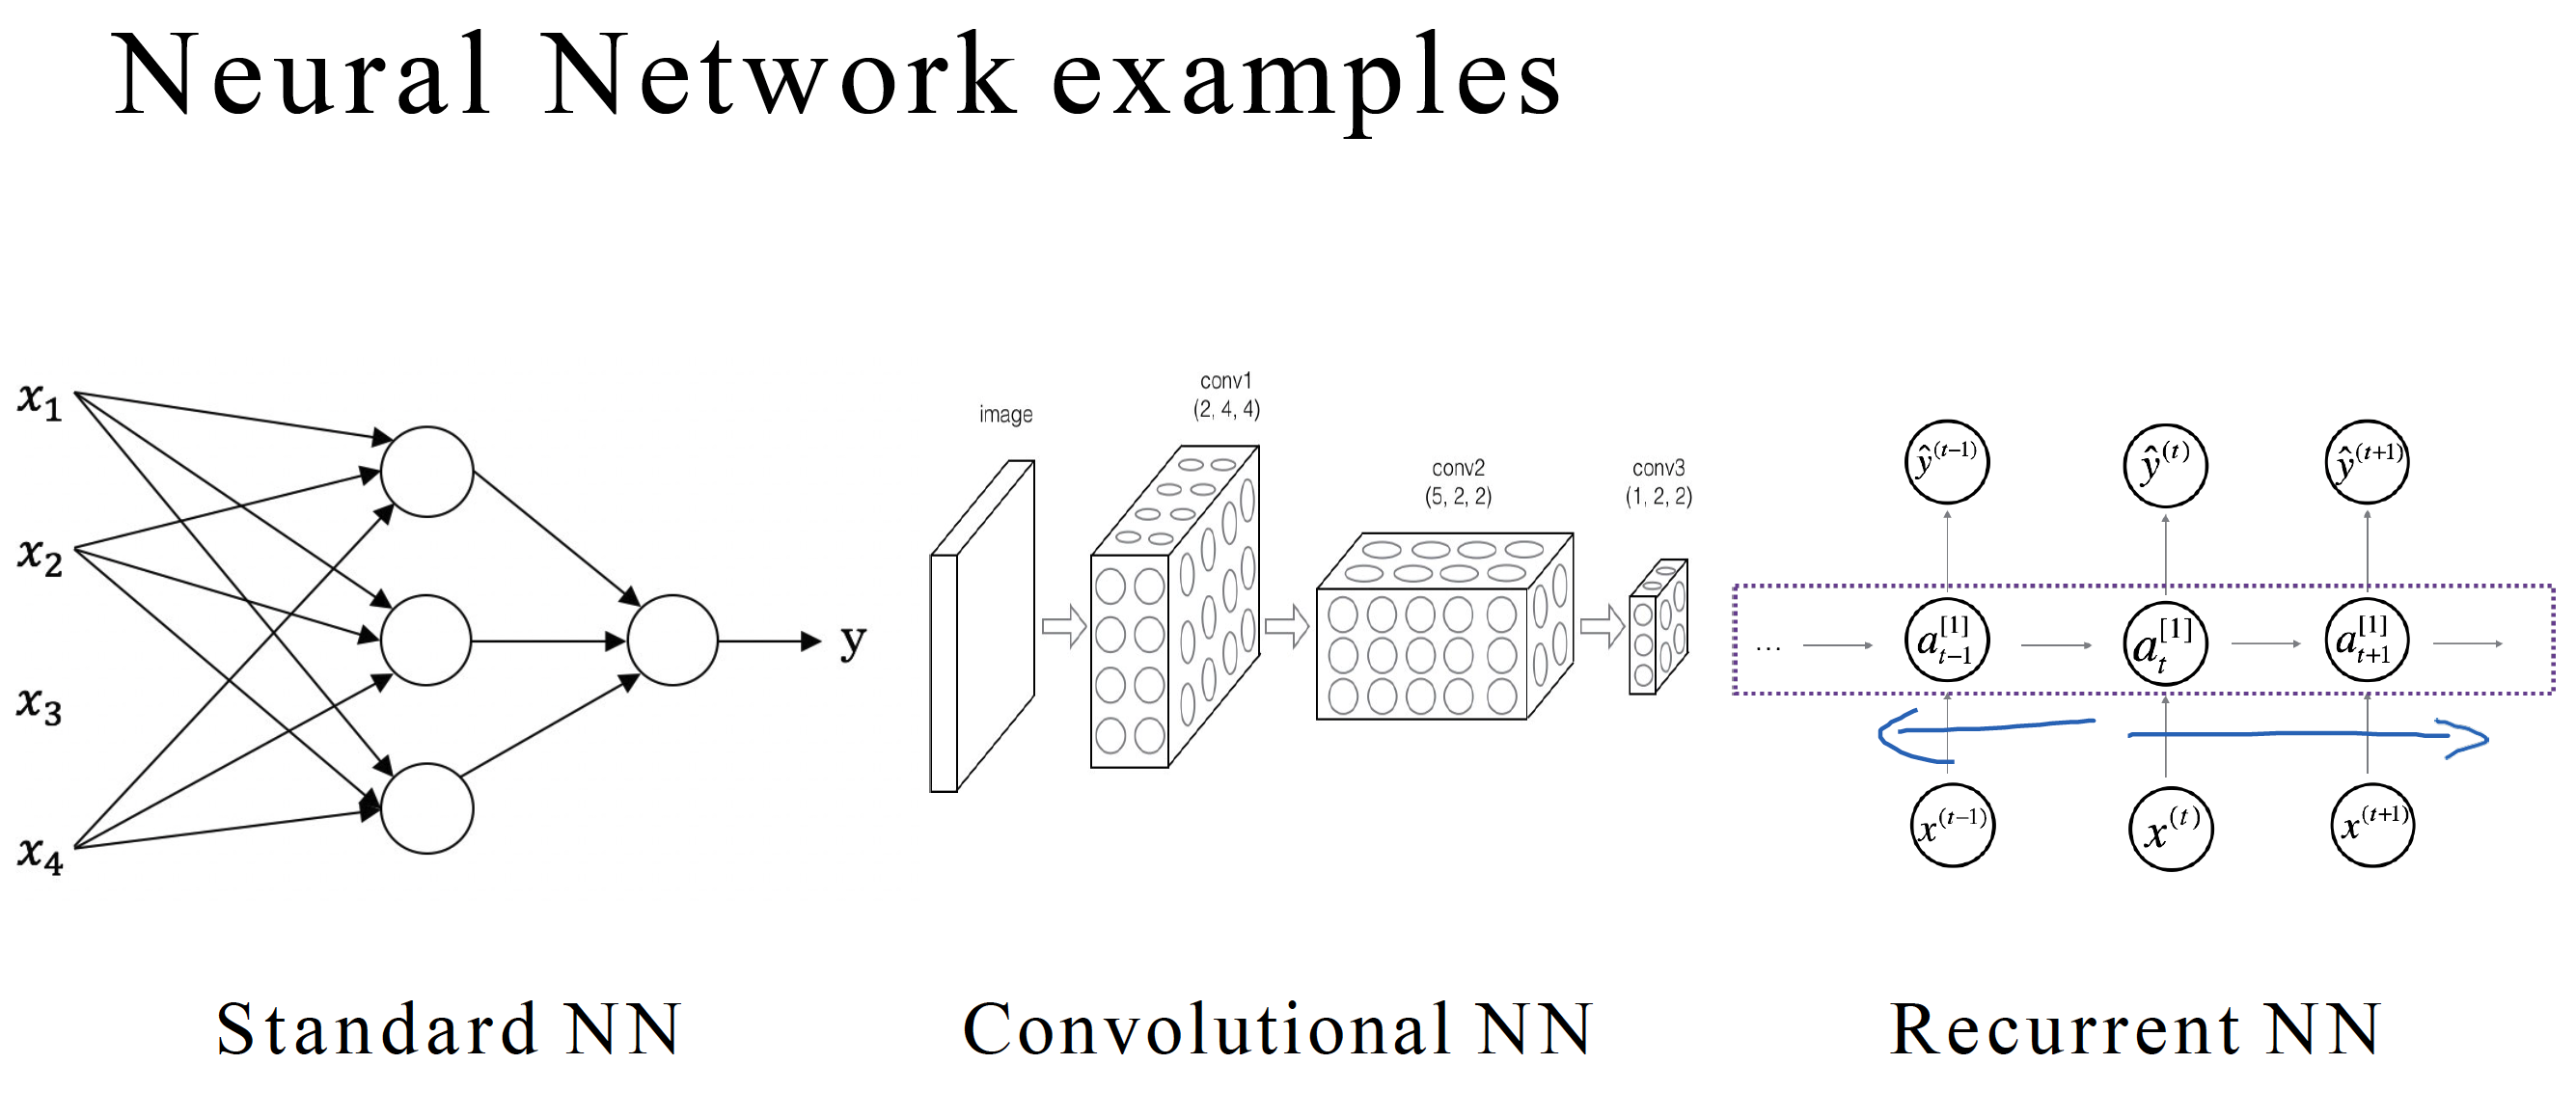
\includegraphics[width=0.75\textwidth]{Images/Neural network examples.png}
	\caption{Neural network examples}
	\label{fig:3}
\end{figure}
\FloatBarrier

\subsection{Why is Deep Learning taking off?}
The rise of deep learning has been fueled by several key factors. One major driver is the abundance of data available for training machine learning models. With the digitization of society, activities performed on digital devices generate vast amounts of data, enabling neural networks to learn from large datasets. Additionally, advancements in hardware, such as GPUs and specialized processors, have facilitated the training of large neural networks by providing faster computation speeds. Algorithmic innovations, like the adoption of the ReLU activation function, have also played a crucial role in accelerating learning processes. By reducing the time required to train models and enabling faster experimentation, these innovations have enhanced productivity and fostered rapid progress in deep learning research. Moving forward, the continued growth of digital data, advancements in hardware technology, and ongoing algorithmic research are expected to further drive improvements in deep learning capabilities. As a result, deep learning is poised to continue evolving and delivering advancements in various applications for years to come.

\begin{funfact}[frametitle=\facttitlep{FunFact}{What's drives Deep Learning}]
Deep Learning took off in the last few years and not before mainly because of great computing power and huge amount of data. These two are the key components for the successes of deep learning. The performance of a neural network improves with more training data.
\end{funfact}

\begin{figure}[h]
	\centering
	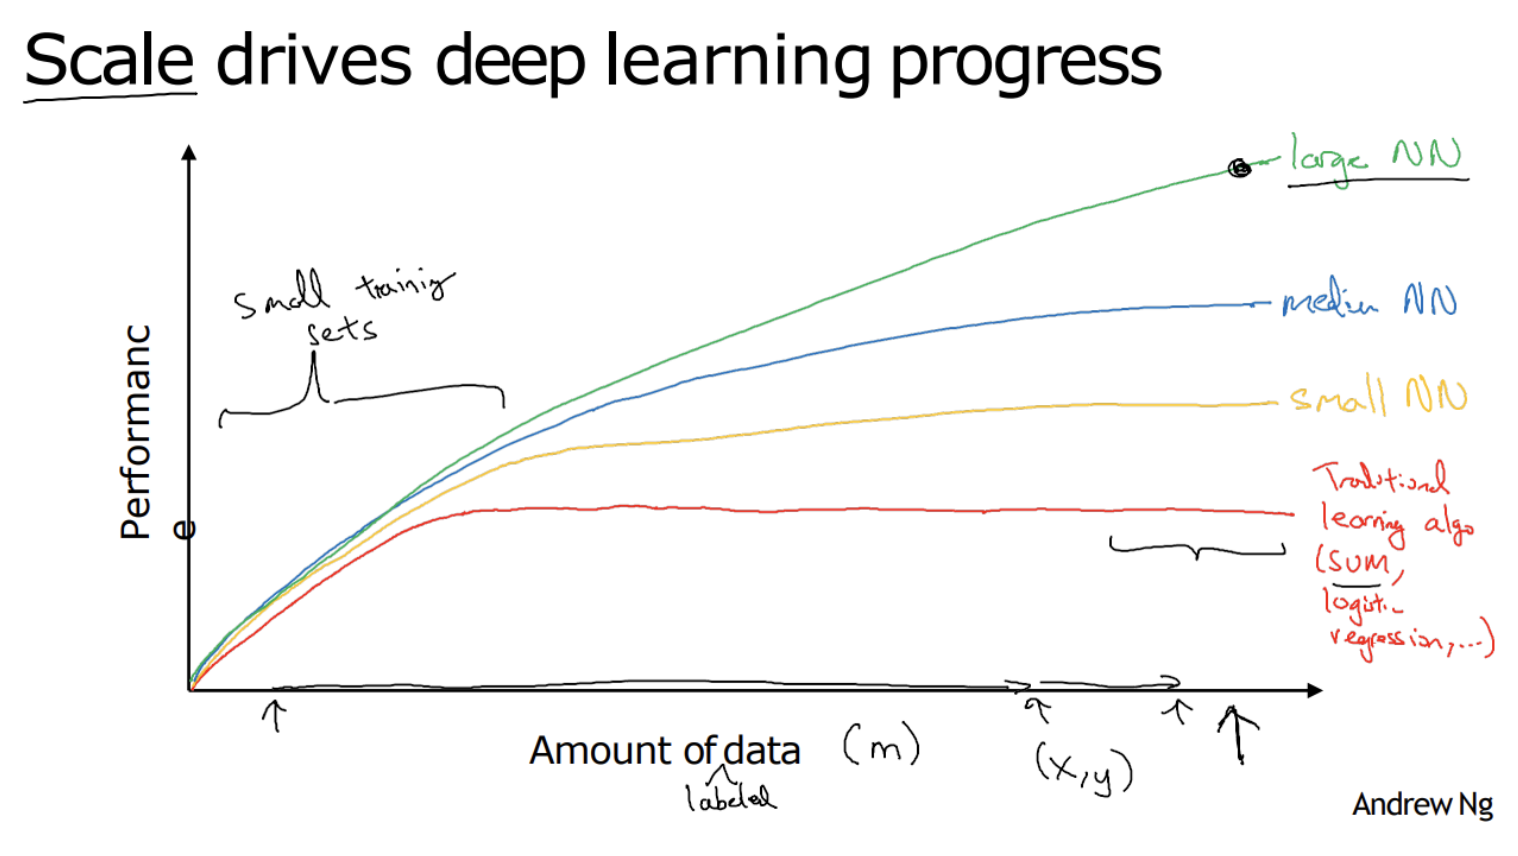
\includegraphics[width=0.75\textwidth]{Images/Scale and neural network.png}
	\caption{Scale drives neural networks}
	\label{fig:4}
\end{figure}
\FloatBarrier

% ------------------ Neural Network Basics -----------------------------%
\section{Neural Network Basics}
\subsection{Logistic Regression as a Neural Network}
Logistic regression is an algorithm for binary classification problem.  In a binary classification problem,  the goal is to train a classifier for which the input is an image represented by a feature vector, $x$, and predicts whether the corresponding label $y$ is 1 or 0. In this case, whether this is a cat image (1) or a non-cat image (0). 

\begin{figure}[h]
	\centering
	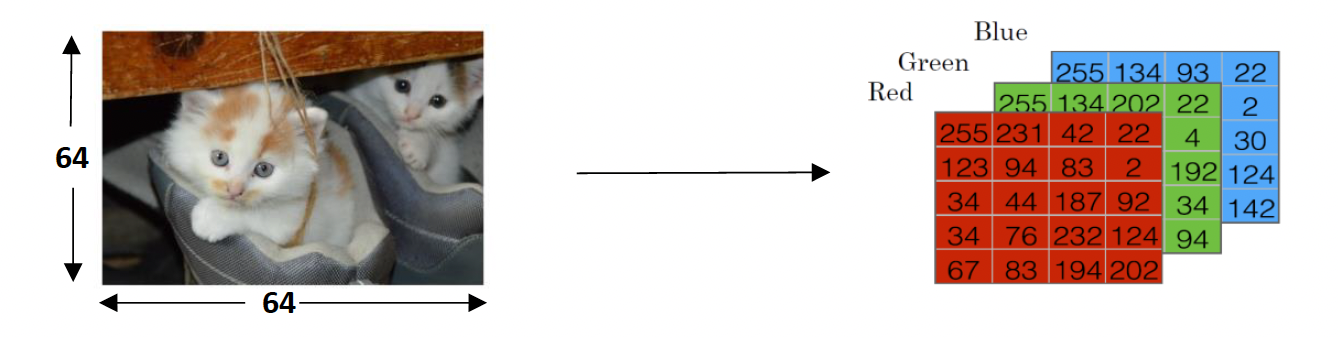
\includegraphics[width=0.95\textwidth]{Images/Binary classification cat example.png}
	\caption{Binary classification - Cat vs Non-Cat}
	\label{fig:5}
\end{figure}
\FloatBarrier

An image is stored in the computer in three separate matrices corresponding to the Red, Green, and Blue color channels of the image. The three matrices have the same size as the image, for example, the resolution of the cat image is 64 pixels x 64 pixels, the three matrices (RGB) are 64 x 64 each. The value in a cell represents the pixel intensity which will be used to create a feature vector of $n$ dimension. In pattern recognition and machine learning, a feature vector represents an image, Then the classifier's job is to determine whether it contain a picture of a cat or not.
To create a feature vector, $x$, the pixel intensity values will be ``unrolled'' or ``reshaped'' for each color. The dimension of the input feature vector $x$ is $n = 64* 64* 3 = 12288$. Hence, we use $n_x = 12288$ to represent the dimensions of the feature vectors. 

\begin{example}
     In binary classification, our goal is to learn a classifier that can input an image represented by this feature vector $x$ and predict whether the corresponding label $y$ is 1 or 0, that is, whether this is a cat image or a non-cat image. 
\end{example}

\begin{figure}[h]
	\centering
	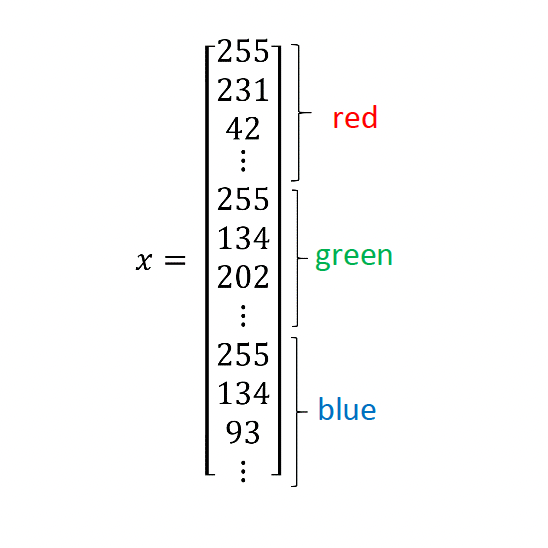
\includegraphics[width=0.35\textwidth]{Images/Reshaped feature vector.png}
	\caption{Reshaped feature vector}
	\label{fig:6}
\end{figure}
\FloatBarrier

\subsubsection{Logistic Regression}
In Logistic regression, the goal is to minimize the error between the prediction and the training data. Given an image represented by a feature vector $x$, the algorithm will evaluate the probability of a cat being in that image.

\begin{equation}
\text{Given}~ x , \hat{y} = P(y=1|x), \text{where}~0 \leq \hat{y} \leq 1
\end{equation}
The parameters used in Logistic regression are:
\begin{itemize}[nosep]
\item The input features vector: $x \in \mathbb{R}^{n_x}$, where $n_x$ is the number of features
\item The training label: $y \in 0,1$
\item The weights: $w \in \mathbb{R}^{n_x}$, where $n_x$ is the number of features
\item The threshold: $b \in \mathbb{R}$
\item The output: $\hat{y} = \sigma*(w^T*x+b)$
\item Sigmoid function: $s = \sigma(w^T*x+b) = \sigma(z)= \frac{1}{1+e^{-z}}$
\end{itemize}
$w^Tx+b$ is a linear function $(ax+b)$, but since we are looking for a probability constraint between $[0,1]$, the sigmoid function is used. The function is bounded between $[0,1]$ as shown in the graph above.
Some observations from the graph:
\begin{enumerate}[nosep]
\item If $z$ is a large positive number, then $\sigma(z) = 1$
\item If $z$ is small or large negative number, then $\sigma(z) = 0$
\item If $z=0$, then $\sigma(z) = 0.5$
\end{enumerate}

\begin{example}
     The difference between the cost function and the loss function for logistic regression is that the loss function computes the error for a single training example while the cost function is the average of the loss functions of the entire training set. 
\end{example}

Logistic regression makes use of the sigmoid function which outputs a probability between 0 and 1. The sigmoid function with some weight parameter $\theta$ or $w$ and some input $x^{(i)}$ is defined as follows. 

\begin{figure}[h]
	\centering
	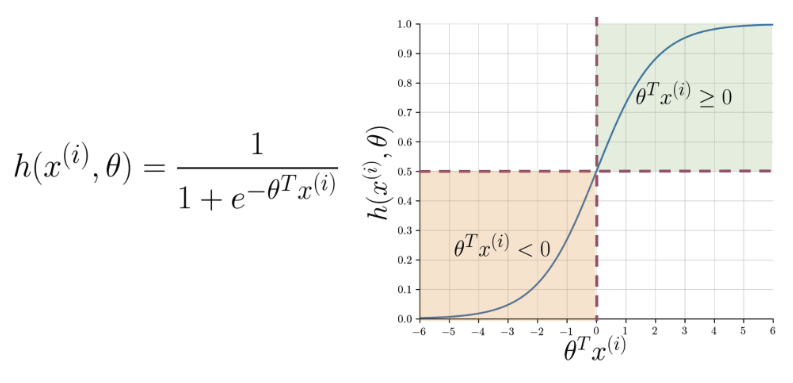
\includegraphics[width=0.85\textwidth]{Images/Logistic with sigmoid fxn.png}
	\caption{Logistic Regression Overview}
	\label{fig:7}
\end{figure}

Note that as $\theta^T x^{(i)}$ i.e.  $w^Tx$ gets closer and closer to $-\infty$ the denominator of the sigmoid function gets larger and larger and as a result, the sigmoid gets closer to 0.  On the other hand, as $\theta^T x^{(i)}$ i.e.  $w^Tx$ gets closer and closer to $\infty$ the denominator of the sigmoid function gets closer to 1 and as a result the sigmoid also gets closer to 1. 

\begin{example}
    When we implement logistic regression,  our job is to try to learn parameters $w$ and $b$ so that $\hat{y}$ becomes a good estimate of the chance of $y$ being equal to one. 
\end{example}

\subsubsection{Logistic Regression Cost function}

The \emph{loss function} ($\mathcal{L}$) is a function we need to define to measure how good our output $\hat{y}$ is when the true label is $y$. The loss function measures how well we are doing on a single training example. \\
\textcolor{RoyalBlue}{$\text{Loss function}~ \Rightarrow~ \mathcal{L}(\hat{y}, y) = - y*log~\hat{y} + (1 - y)*log(1 - \hat{y})$}

The \emph{cost function} ($\mathcal{J}$), which measures how we are doing on the entire training set. So the cost function, which is applied to your parameters $w$ and $b$, is going to be the average, really one of the $m$ of the sum of the loss function apply to each of the training examples.  \\
\textcolor{RoyalBlue}{$\text{Cost function}~  \Rightarrow~ \mathcal{J}(w, b) = \frac{1}{m} \sum_{i=1}^m \mathcal{L}(\hat{y}, y) = - \frac{1}{m}  \sum_{i=1}^m[y^{(i)}*log~\hat{y}^{(i)} + (1 - y^{(i)})*log(1 - \hat{y}^{(i)})]$}

\begin{figure}[h]
	\centering
	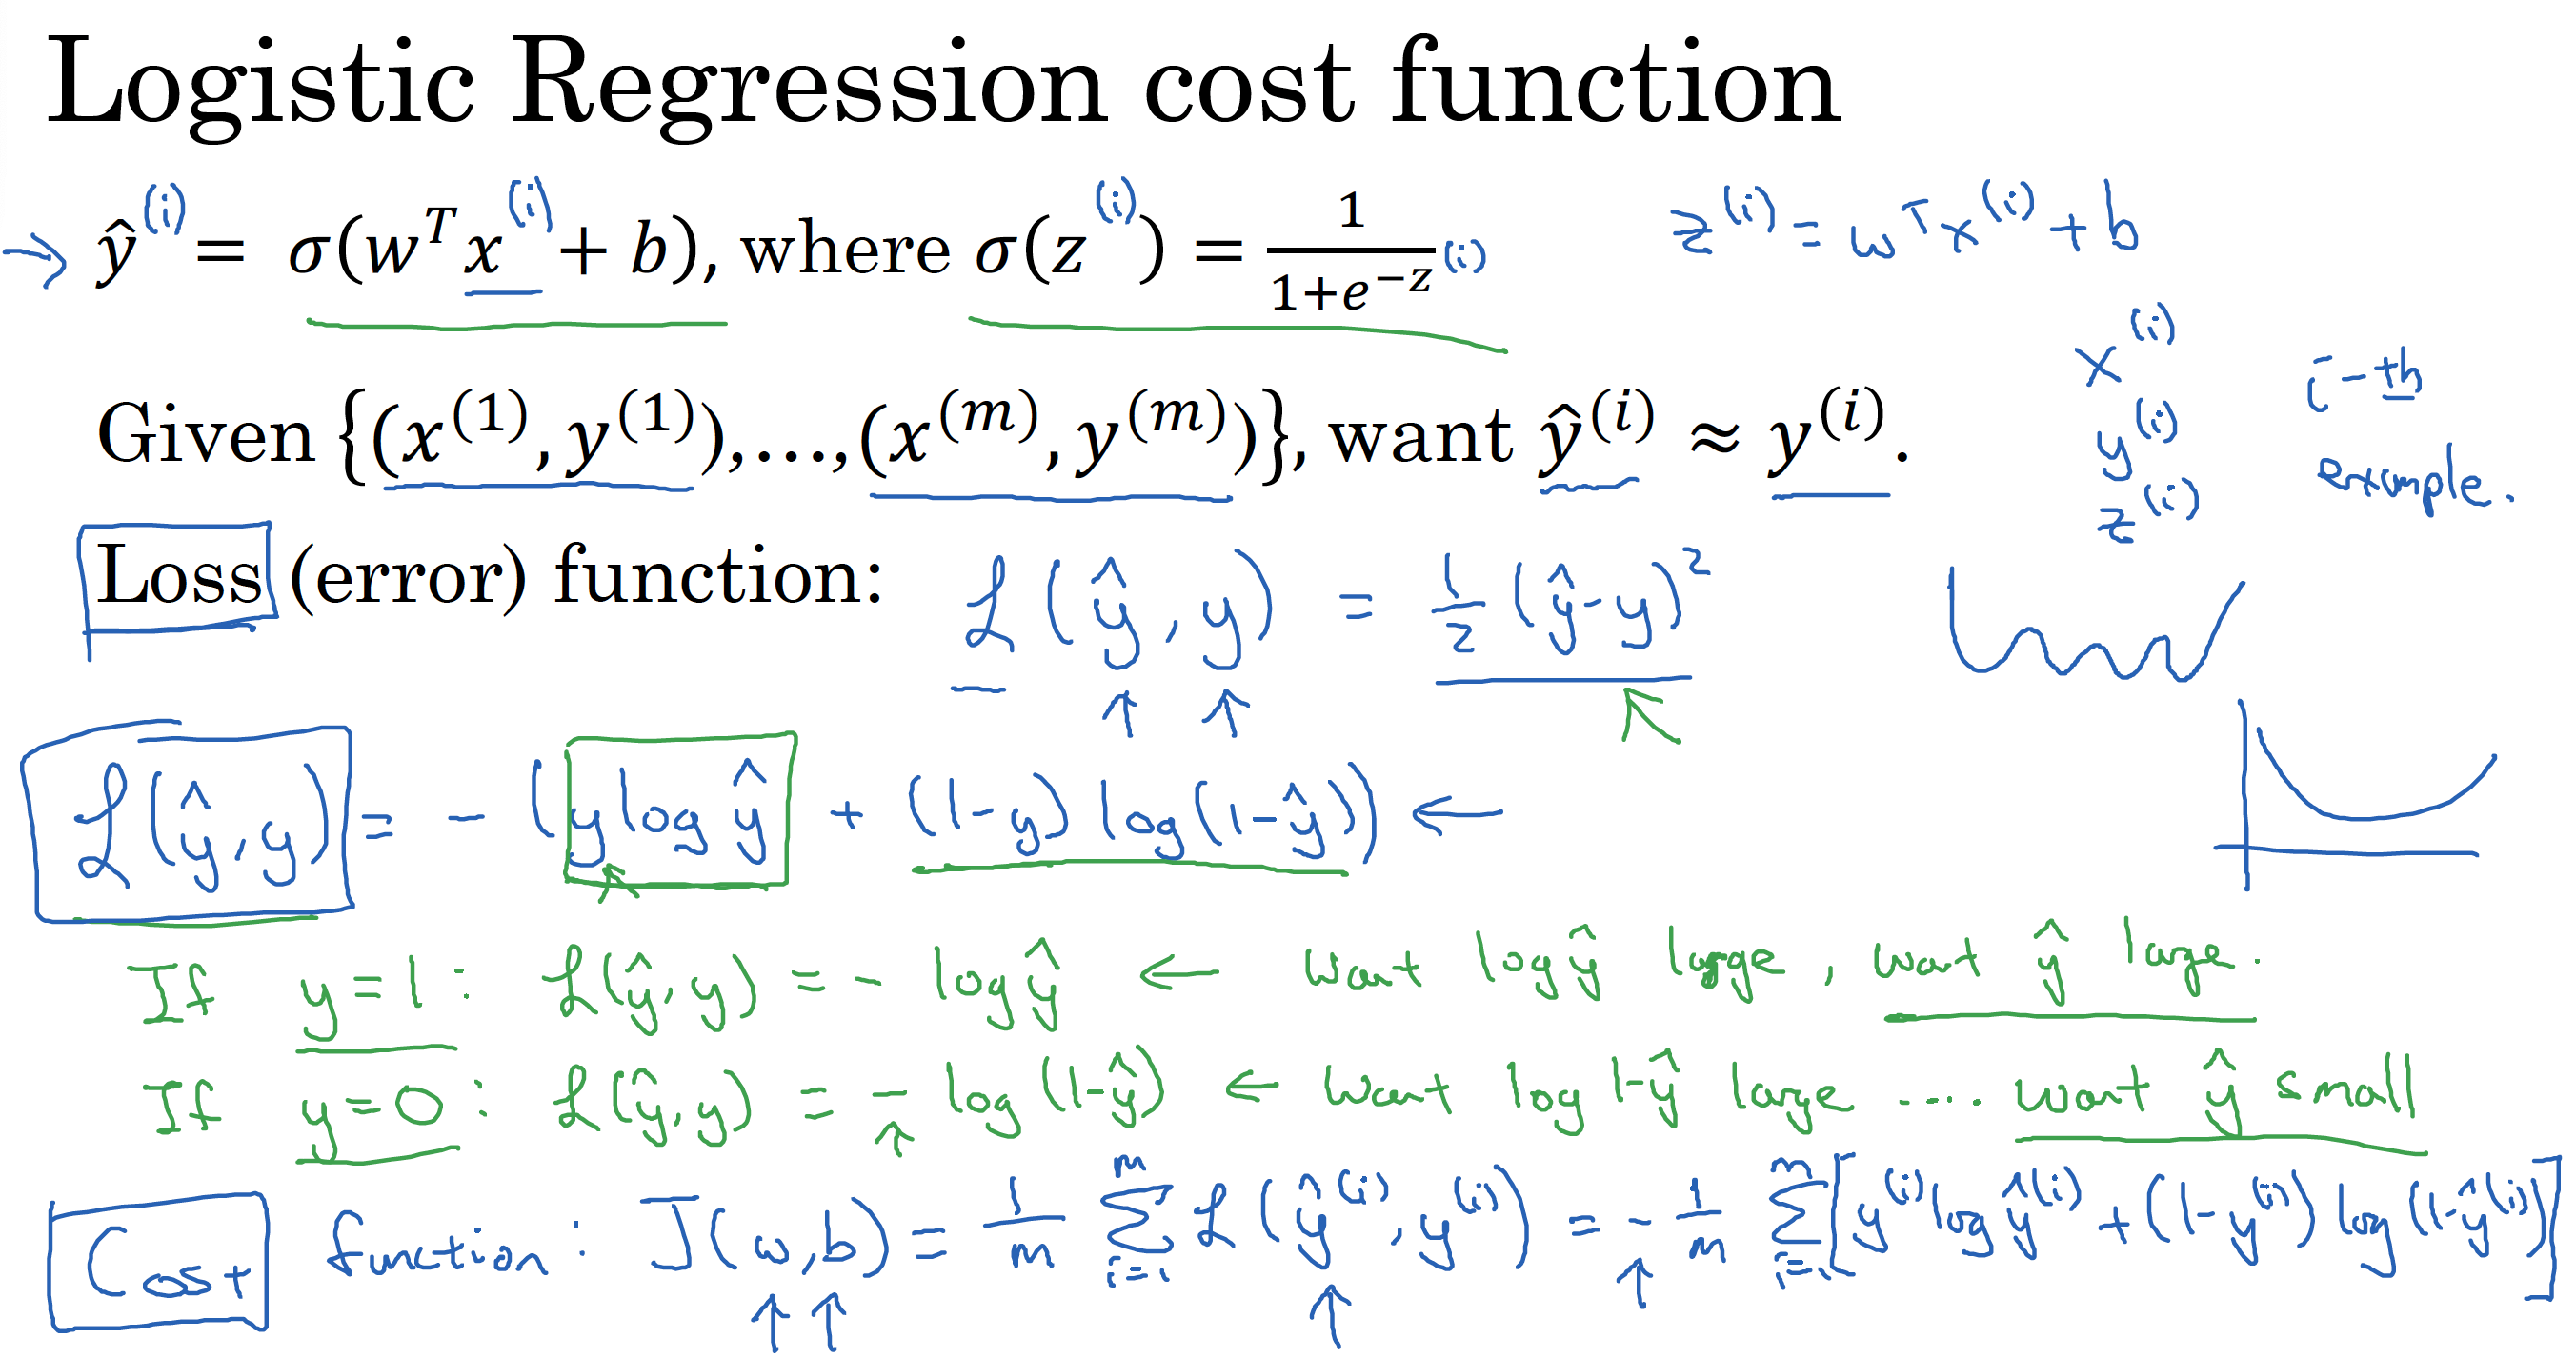
\includegraphics[width=0.85\textwidth]{Images/Cost function.png}
	\caption{Logistic Regression Cost function}
	\label{fig:8}
\end{figure}
\FloatBarrier

\begin{figure}[h]
	\centering
	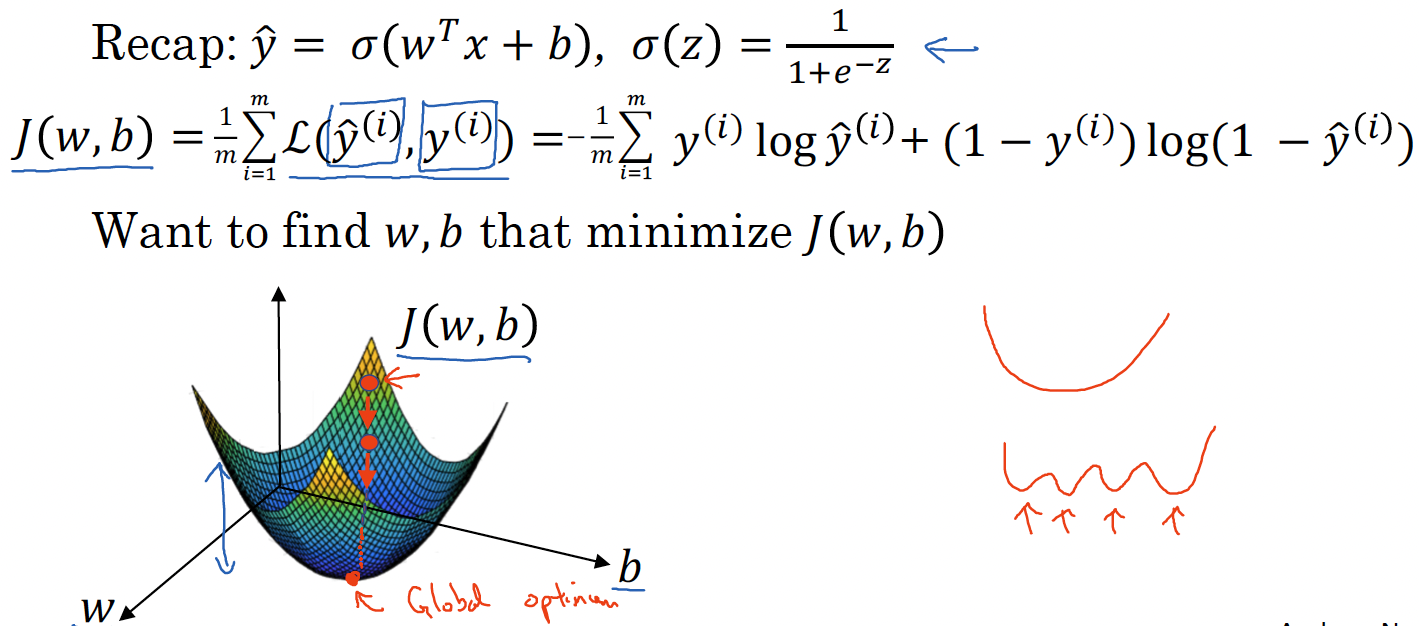
\includegraphics[width=0.85\textwidth]{Images/Gradient descent plot.png}
	\caption{Gradient Descent}
	\label{fig:9}
\end{figure}
\FloatBarrier

In logistic regression, you use the cost function $\mathcal{J}(w, b)$ to measure how well your parameters perform on the entire training set. The goal is to minimize $ \mathcal{J}(w, b)$ using gradient descent, which iteratively updates the parameters by moving in the direction of steepest descent. Because the cost function is convex, gradient descent will converge to the global minimum, regardless of initialization.

\begin{figure}[h]
	\centering
	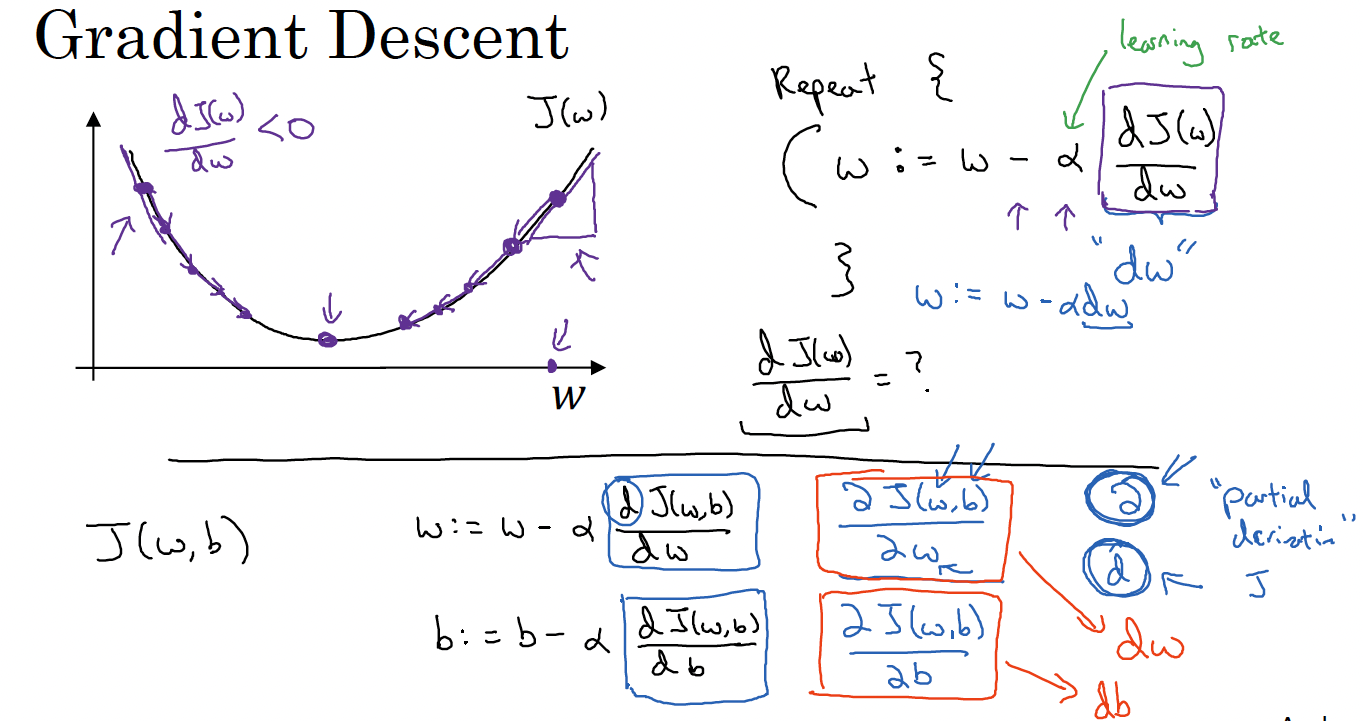
\includegraphics[width=0.85\textwidth]{Images/Gradient descent.png}
	\caption{Gradient descent Optimization}
	\label{fig:10}
\end{figure}
\FloatBarrier

\subsection{Gradient Descent}
\begin{funfact}
Imagine you're on top of a big hill where the goal is to get to the lowest point.
Here's how you would do it:

\begin{itemize}[nosep]
\item Look around you to see which way the ground slopes down the most. 
\item Take a step in that direction. 
\item Now that you're in a new spot, look around again to see which way is downhill.
\item Take another step in that direction. 
\item Keep doing this over and over: look for the downhill direction, then take a step. 
\item Eventually, you'll reach a point where there's no more downhill to go. You're at the bottom!
\end{itemize}

This is basically what gradient descent does. The ``hill'' is like a mathematical function we're trying to minimize. ``Looking around'' is like calculating the gradient (which tells us which direction is downhill).``Taking a step'' is like updating our parameters (our position on the hill). We keep doing this until we can't go any lower (we've reached the minimum of the function).

The trick is to not take steps that are too big (or you might overshoot the bottom) or too small (or it will take forever to get there). In the algorithm, we control this with something called the ``learning rate''. That's gradient descent! It's a way of finding the lowest point by always moving downhill, little by little.
\end{funfact}

\newpage
\textbf{Gradient descent} is an optimization technique used to minimize a function, often applied in machine learning for model training. The algorithm starts with an initial guess for the parameters and iteratively updates them by moving in the direction of the negative gradient (the direction of steepest descent) of the function, until it reaches a local minimum. The step size, or learning rate, controls how big each move is.

The gradient descent update rule is:

\[
\theta_{\text{new}} = \theta_{\text{old}} - \alpha \nabla J(\theta)
\]
where:
\begin{itemize}
    \item \( \theta \) are the parameters we want to optimize.
    \item \( \alpha \) is the learning rate (step size).
    \item \( \nabla J(\theta) \) is the gradient of the cost function \( J(\theta) \) with respect to \( \theta \).
\end{itemize}
This rule ensures that we move in the direction of the steepest descent, reducing the value of \( J(\theta) \) with each iteration.

\subsubsection{Why It Works}
The gradient of a function points in the direction of the steepest ascent. By moving in the opposite direction of the gradient, the function value decreases, eventually reaching a local or global minimum. As the gradient approaches zero, the parameter values converge toward the minimum.

\subsubsection{Pseudocode}
Below is the pseudocode for gradient descent in simple terms:

\begin{lstlisting}
initialize $\theta$ (e.g., random values) 
choose learning rate $\alpha$
repeat until convergence:
    $\quad$ compute gradient $\nabla J(\theta)$
    $\quad$ update $\theta: \theta = \theta - \alpha * \nabla J(\theta)$
\end{lstlisting}

\begin{algorithm}
\caption{Gradient Descent}
\begin{flushleft}
\textbf{Input:} Initial parameter $\theta^0$, gradient of loss function $\nabla J(\theta)$, learning rate $\alpha$, tolerance $\epsilon$, maximum iterations $max\_iter$\\
\textbf{Output:} Optimized parameter $\theta$\\

$iter \leftarrow 0$\\
\textbf{while} $iter < max\_iter$ \textbf{do}\\
\hspace{1em}Compute $\nabla J(\theta)$\\
\hspace{1em}\textbf{if} $\|\nabla J(\theta)\| < \epsilon$ \textbf{then}\\
\hspace{2em}\textbf{break}\\
\hspace{1em}\textbf{end if}\\
\hspace{1em}$\theta \leftarrow \theta - \alpha \nabla J(\theta)$\\
\hspace{1em}$iter \leftarrow iter + 1$\\
\textbf{end while}\\
\textbf{return} $\theta$
\end{flushleft}
\end{algorithm}

The process repeats until the gradient is close to zero, indicating the function has been minimized.

\begin{example}
Gradient descent is an optimization algorithm used to minimize the cost function of a model by iteratively adjusting the model's parameters. The goal is to find the values of the parameters (like weights in a machine learning model) that minimize the cost function, which measures how well the model fits the data.
\end{example}

\subsubsection*{How Gradient Descent Works:}
\begin{enumerate}
    \item \textbf{Initialize Parameters:} Start with an initial guess for the parameters (e.g., weights). This can be a set of random values or zeros.
    
    \item \textbf{Calculate the Gradient:} Compute the gradient (i.e., the partial derivative) of the cost function with respect to each parameter. The gradient indicates the direction of the steepest increase in the cost function.
    
    \item \textbf{Update the Parameters:} Adjust the parameters in the opposite direction of the gradient (i.e., the direction that reduces the cost function). The size of the step taken is controlled by a learning rate, a hyperparameter that determines how big the steps are.
    
    \[
    \text{new parameter} = \text{current parameter} - \text{learning rate} \times \text{gradient}
    \]
    
    \item \textbf{Repeat:} Continue recalculating the gradient and updating the parameters until the algorithm converges, meaning the changes in the cost function become very small, indicating that a minimum has been reached.
\end{enumerate}

\begin{funfact}[frametitle=\facttitlep{FunFact}{Computation Graph}]
The computation graph organizes a computation from left-to-right computation. Through a left-to-right pass, we can compute the value of $\mathcal{J}$. In order to compute derivatives there'll be a right-to-left pass, kind of going in the opposite direction called backwards propagation. That would be most natural for computing the derivatives. 
\end{funfact}

\textbf{Forward Propagation}: Computes the output $y$ from the input $X$ by passing through the network layers. \\
\textbf{Backward propagation} adjusts the network's parameters (weights and biases) by propagating the error backward from the output to the input, using the gradients to minimize the loss.

% ------------------ Shallow Neural Network -----------------------------%
\section{Shallow Neural Network}
\subsection{Neural Network Representation}
A neural network is a machine learning model inspired by the human brain. It consists of layers of interconnected nodes (neurons) where each connection has a weight, representing its importance. Neural networks process input data by passing it through these layers, applying activation functions to transform the data, and adjusting the weights based on the output error during training. The goal is to minimize the error and improve the model's predictions. Neural networks are widely used in tasks like image recognition, language processing, and complex data modeling.

\begin{figure}[h]
	\centering
	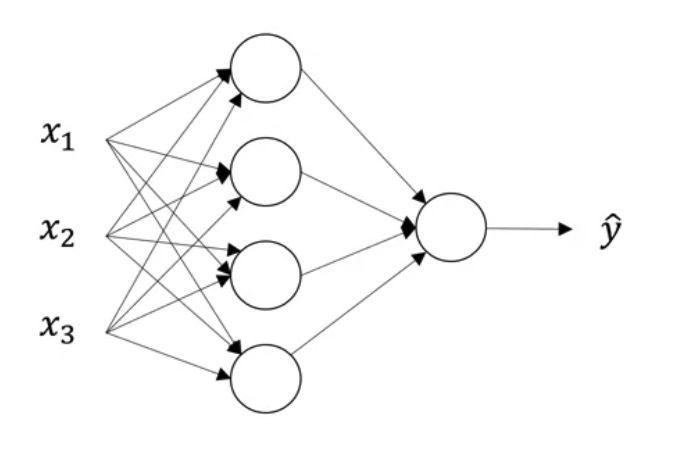
\includegraphics[width=0.65\textwidth]{Images/Shallow Neural Network.png}
	\caption{Shallow Neural Network}
	\label{fig:11}
\end{figure}

\subsection{Neural Network Structure}
A simple neural network has similar structure as a linear classifier:
\begin{itemize}[nosep]
\item A neuron takes inputs from other neurons (-> input into linear classifier)
\item The inputs are summed in a weighted manner (-> weighted sum)
	\begin{itemize}[label={\ding{224}}]
		\item Learning is through a modification of the weights (gradient descent in the case of NN)
	\end{itemize}
\item If it receives enough inputs, it “fires” (if it exceeds the threshold or weighted sum plus bias is high enough)
\item The output of a neuron can be modulated by a non linear function (e.g sigmoid).
\end{itemize}

\begin{figure}[h]
	\centering
	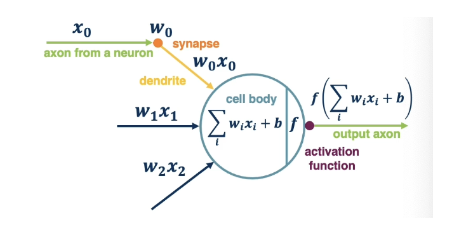
\includegraphics[width=0.75\textwidth]{Images/Activation function.png}
	\caption{Structure of a simple neural network}
	\label{fig:12}
\end{figure}

A neural network consists of three primary layers: input, hidden, and output layers as shown in \textbf{Fig. \ref{fig:13}}.

\begin{figure}[h]
	\centering
	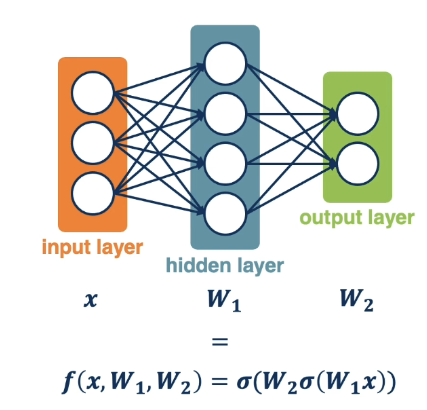
\includegraphics[width=0.5\textwidth]{Images/Layers in a neural network.png}
	\caption{Layers in a neural network}
	\label{fig:13}
\end{figure}

\begin{figure}[h]
	\centering
	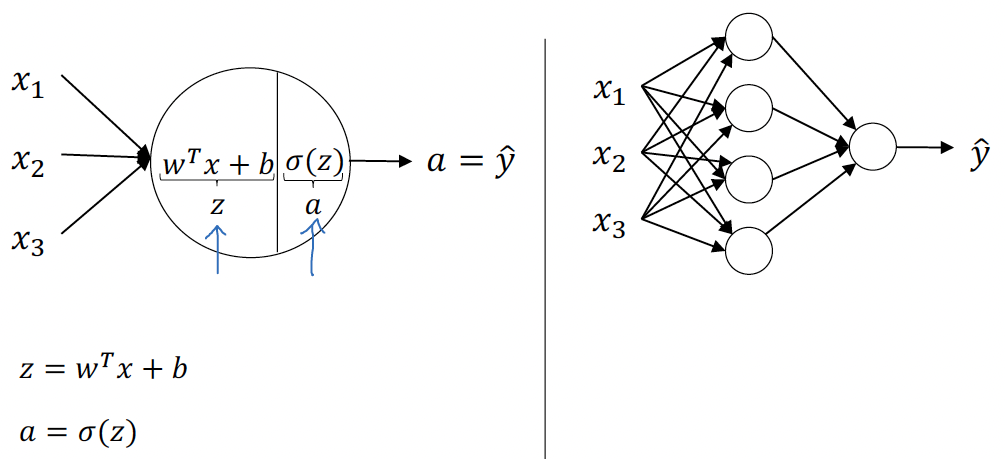
\includegraphics[width=0.85\textwidth]{Images/Neural Network Representation.png}
	\caption{Neural Network Representation}
	\label{fig:14}
\end{figure}
\FloatBarrier

\subsubsection{Input Layer}
The \textbf{input layer} is responsible for taking in the features of the data. For example, features \( x_1, x_2, x_3 \) are passed into the network in \textbf{Fig. \ref{fig:14}}, and these values are referred to as the \textit{activations} of the input layer, denoted \( A^{[0]} \).

\subsubsection{Hidden Layer}
The \textbf{hidden layer} processes the input features. It is called \textit{hidden} because, during training, the true values for these nodes are not seen in the training data. The activations of this layer are denoted \( A^{[1]} \), where each node \( A^{[1]}_i \) represents an activation value computed using a weight matrix \( W^{[1]} \) and bias vector \( b^{[1]} \). For example, if there are four hidden units, \( A^{[1]} \) will be a 4-dimensional vector.

\subsubsection{Output Layer}
The \textbf{output layer} produces the final prediction \( \hat{y} \), based on the activations from the hidden layer. The output is represented as \( A^{[2]} \), a single scalar value in this example.

\subsubsection{Notation}
We use the following notations to represent the activations in different layers:
\begin{itemize}
    \item \( A^{[0]} \): Activations of the input layer.
    \item \( A^{[1]} \): Activations of the hidden layer.
    \item \( A^{[2]} \): Output, representing \( \hat{y} \).
\end{itemize}

In the neural network in \textbf{Fig. \ref{fig:14}}, each layer has associated weight matrices and biases:
\begin{itemize}
    \item \( W^{[1]} \) is a \( 4 \times 3 \) matrix (4 hidden units, 3 input features).
    \item \( b^{[1]} \) is a \( 4 \times 1 \) vector (for 4 hidden units).
    \item \( W^{[2]} \) is a \( 1 \times 4 \) matrix (1 output unit, 4 hidden units).
    \item \( b^{[2]} \) is a \( 1 \times 1 \) scalar (for the output unit).
\end{itemize}

While this neural network has three layers (input, hidden, output), it is commonly referred to as a \textbf{two-layer network} because the input layer is not counted. Therefore, the hidden layer is called \textit{layer 1} and the output layer \textit{layer 2}.

\subsubsection{Training}
The parameters \( W \) and \( b \) are optimized during training to minimize the error between the predicted output \( \hat{y} \) and the actual output \( y \). In this process, the neural network learns the best weights and biases for making accurate predictions.

\subsection{Activation Functions}
Activation functions are mathematical equations that determine the output of a neural network node. They introduce non-linearity into the model, enabling the network to learn complex patterns. Below are some common activation functions used in neural networks:

\subsubsection{1. Sigmoid Function}
The \textbf{sigmoid} activation function is defined as:
\[
a = \sigma(x) = \frac{1}{1 + e^{-z}}
\]
It compresses input values to a range between 0 and 1, making it useful for models that need probabilities as output or binary classification. However, it suffers from the \textit{vanishing gradient problem}, where gradients become very small, slowing down learning.

\subsubsection{2. Tanh Function}
The \textbf{tanh} activation function is defined as:
\[
a = \text{tanh}(z) = \frac{e^{z} - e^{-z}}{e^{z} + e^{-z}}
\]
It outputs values between -1 and 1, centered around zero, making learning more efficient in some cases. Like sigmoid, it also suffers from vanishing gradients but it is superior to the sigmoid function for hidden layers.

\subsubsection{3. ReLU (Rectified Linear Unit)}
The \textbf{ReLU} activation function is defined as:
\[
a = \text{ReLU}(z) = \max(0, z)
\]
ReLU is simple and efficient, especially in deep networks, because it allows faster convergence. The downside is that it can cause ``dead neurons'' (neurons that output 0 for all inputs), which may stop learning in certain neurons.

\subsubsection{4. Leaky ReLU}
The \textbf{Leaky ReLU} activation function is defined as:
\[
a = \max(0.01z, z)
\]
The Leaky ReLU adresses the ReLU's zero-gradient issue by allowing small negative values. Generally works better than ReLU but is used less frequently.

\subsubsection{5. Softmax Function}
The \textbf{softmax} function is commonly used in the output layer for classification tasks. It converts raw outputs (logits) into probabilities:
\[
\text{Softmax}(z_i) = \frac{e^{z_i}}{\sum_{j}e^{z_j}}
\]
This is useful for multi-class classification, ensuring the sum of output probabilities equals 1.

\subsubsection{Choosing an Activation Function}
\textbf{ReLU} is popular for hidden layers in deep neural networks due to its simplicity and efficiency.  \textbf{Sigmoid} and \textbf{tanh} are useful in smaller networks or specific scenarios but less common in modern deep networks.  \textbf{Softmax} is used in the output layer for multi-class classification tasks.
\begin{itemize}
    \item \textbf{Output Layer}: Use \textbf{Sigmoid} for binary classification.
    \item \textbf{Hidden layers}: \textbf{ReLU} is the default choice, though \textbf{tanh} can also be used effectively.
    \item \textbf{Learning Efficiency}: \textbf{ReLU} and \textbf{Leaky ReLU} often result in faster learning compared to sigmoid or tanh, as their gradients do not saturate easily.
\end{itemize}

Each activation function has its specific use cases depending on the task and network architecture.

\begin{figure}[h]
	\centering
	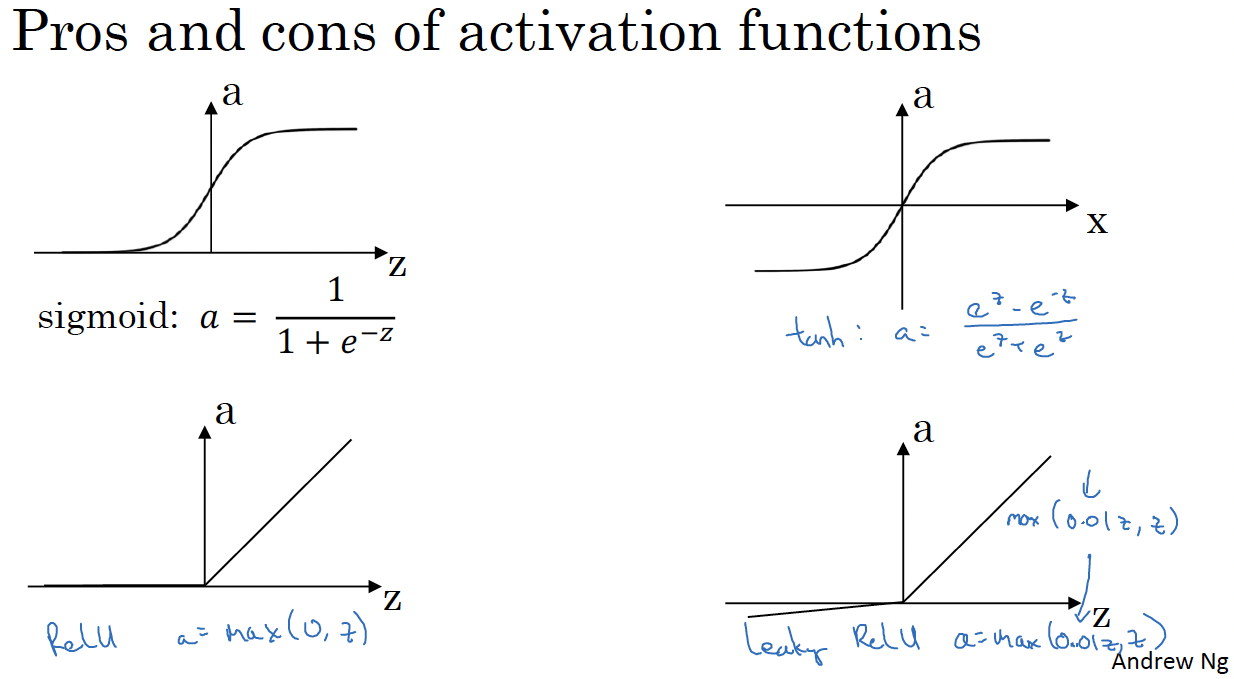
\includegraphics[width=0.85\textwidth]{Images/Activation functions.png}
	\caption{Activation Functions in Neural Networks}
	\label{fig:15}
\end{figure}
\FloatBarrier

% ------------------ Deep Neural Network ---------------------------%
\section{Deep Neural Network}
% ------------ Deep L-layer Neural Network -----------------%
\subsection{Deep L-layer Neural Network}
A \textbf{Deep Neural Network (DNN)} is a type of artificial neural network that contains multiple layers between the input and output layers. These intermediate layers, known as \textit{hidden layers}, allow the network to learn more complex patterns and representations from the data.

\subsubsection{Key Characteristics of Deep Neural Networks:}
\begin{enumerate}
    \item \textbf{Multiple Hidden Layers}:
    \begin{itemize}
        \item Unlike shallow networks (such as logistic regression or simple neural networks with a single hidden layer), a deep neural network has multiple hidden layers. The more hidden layers a network has, the ``deeper'' it is.
        \item \textit{Example}: A network with 3 hidden layers and an output layer would have a depth of 4 (input layer not counted in depth).
    \end{itemize}

    \item \textbf{Ability to Learn Complex Functions}:
    \begin{itemize}
        \item By stacking multiple layers, each layer in a DNN extracts features or patterns from the previous layer's output. This enables the network to learn complex and abstract representations of data.
        \item Shallow networks are often limited in their ability to model complex relationships, while DNNs can learn hierarchical patterns.
    \end{itemize}

    \item \textbf{Forward and Backward Propagation}:
    \begin{itemize}
        \item \textbf{Forward Propagation}: Data passes through each layer of the network, transforming via weights, biases, and activation functions, until reaching the output layer.
        \item \textbf{Backward Propagation (Backpropagation)}: The network adjusts the weights and biases by calculating errors and gradients to minimize the loss function. This allows the network to learn from the data.
    \end{itemize}

    \item \textbf{Applications}:
    \begin{itemize}
        \item DNNs are widely used in areas such as image recognition, natural language processing, speech recognition, and more.
        \item \textit{For instance}, DNNs power technologies like self-driving cars, facial recognition, and voice assistants.
    \end{itemize}

    \item \textbf{Deep vs. Shallow Networks}:
    \begin{itemize}
        \item \textbf{Shallow Network}: A neural network with one or very few hidden layers (e.g., logistic regression can be viewed as a one-layer network).
        \item \textbf{Deep Network}: A network with multiple hidden layers, enabling it to learn from more complex data.
    \end{itemize}
\end{enumerate}

\begin{example}
A deep neural network is a powerful tool for learning from data with multiple hidden layers, making it well-suited for complex tasks that require sophisticated pattern recognition. The depth of the network enables it to model intricate relationships between inputs and outputs that shallow models often cannot handle effectively.
\end{example}

\subsubsection{Notation to describe a Deep Neural Network}
\textbf{Fig. \ref{fig:16}} shows a four-layer neural network consisting of three hidden layers. The number of units in each layer of the neural network is 5, 5, 3, and 1, respectively.  
\begin{figure}[h]
	\centering
	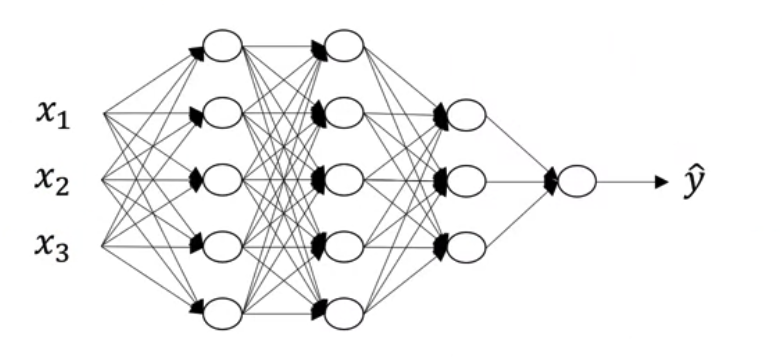
\includegraphics[width=0.85\textwidth]{Images/Deep Neural Network.png}
	\caption{Deep Neural Networks with 5 hidden layers}
	\label{fig:16}
\end{figure}
\FloatBarrier

Let: \\
\begin{itemize}
    \item \( L \): Represents the total number of layers in the network. For this network, \( L = 4 \).
    \item \( n^{[l]} \): Represents the number of units (or nodes) in layer \( l \).
    \begin{itemize}
        \item Example:
        \begin{itemize}
            \item \( n^{[0]} = n_x = 3 \) (input layer).
            \item \( n^{[1]} = 5 \), \( n^{[2]} = 5 \), \( n^{[3]} = 3 \) (hidden layers).
            \item \( n^{[4]} = n^{[L]} = 1 \) (output layer).
        \end{itemize}
    \end{itemize}
    \item \( a^{[l]} \): Denotes the activations of layer \( l \).
    \begin{itemize}
        \item \( a^{[0]} = x \): Activations in the input layer, equivalent to the input features.
        \item \( a^{[L]} = \hat{y} \): Activations in the final layer, equivalent to the predicted output.
    \end{itemize}
    \item \( W^{[l]} \): Denotes the weights for computing \( z^{[l]} \) in layer \( l \).
    \item \( b^{[l]} \): Denotes the biases for computing \( z^{[l]} \) in layer \( l \).
\end{itemize}

\subsubsection*{Activation Functions}
In forward propagation, the activation in layer \( l \), \( a^{[l]} \), is computed as:
\[
a^{[l]} = g(z^{[l]}),
\]
where \( g \) is the activation function, and \( z^{[l]} \) depends on \( W^{[l]} \) and \( b^{[l]} \).

\subsubsection*{Summary of Relationships}
\begin{itemize}
    \item The input layer (\( l = 0 \)): \( a^{[0]} = x \).
    \item The output layer (\( l = L \)): \( a^{[L]} = \hat{y} \) (the network's prediction).
    \item Each layer computes \( z^{[l]} \) using weights (\( W^{[l]} \)) and biases (\( b^{[l]} \)).
\end{itemize}

% ------------ Forward propagation in Deep Neural Network -----------------%
\subsection{Forward propagation in a Deep Neural Network}
Forward propagation in a deep neural network involves passing the input data through the network, layer by layer, to compute the output prediction. Below are the steps to carry out forward propagation:

\subsubsection*{Steps for Forward Propagation}

\begin{enumerate}
    \item \textbf{Input Layer Initialization}:
    \begin{itemize}
        \item Denote the input features as \( x \).
        \item The activations of the input layer are \( a^{[0]} = x \).
    \end{itemize}

    \item \textbf{Layer-wise Computation}: 
	\begin{itemize}
		\item For each layer \( l \) from \( 1 \) to \( L \) (the total number of layers):
		\begin{enumerate}
	        \item \textbf{Linear Combination}: Compute the pre-activation \( z^{[l]} \):
	        \[
	        z^{[l]} = W^{[l]} a^{[l-1]} + b^{[l]},
	        \]
	        where:
	        \begin{itemize}
	            \item \( W^{[l]} \) is the weight matrix for layer \( l \),
	            \item \( b^{[l]} \) is the bias vector for layer \( l \),
	            \item \( a^{[l-1]} \) are the activations from the previous layer.
	        \end{itemize}
	
	        \item \textbf{Activation Function}: Apply an activation function \( g^{[l]} \) to \( z^{[l]} \) to compute the activations \( a^{[l]} \):
	        \[
	        a^{[l]} = g^{[l]}(z^{[l]}).
	        \]
	        The activation function could be ReLU, sigmoid, tanh, or softmax, depending on the task and the layer type.
	   	 \end{enumerate}
	\end{itemize}
    
    \item \textbf{Output Layer}:
    \begin{itemize}
        \item At the final layer \( L \), compute the prediction:
        \[
        a^{[L]} = \hat{y}.
        \]
        \item If it's a regression problem, \( \hat{y} \) is a continuous value (e.g., no activation or linear activation).
        \item For classification, \( \hat{y} \) might involve a sigmoid or softmax activation.
    \end{itemize}
\end{enumerate}

\subsubsection*{Algorithm}

Given \( x \) as input, perform the following:
\begin{itemize}
    \item Initialize \( a^{[0]} = x \).
    \item For \( l = 1 \) to \( L \):
    \begin{itemize}
        \item Compute \( z^{[l]} = W^{[l]} a^{[l-1]} + b^{[l]} \).
        \item Compute \( a^{[l]} = g^{[l]}(z^{[l]}) \).
    \end{itemize}
    \item Return \( a^{[L]} = \hat{y} \), the final prediction.
\end{itemize}

\subsubsection*{Example}

Consider a network with:
\begin{itemize}
    \item Input: \( x \) (dimension: \( n_x \)),
    \item Hidden layers: two layers with ReLU activation,
    \item Output layer: one node with sigmoid activation.
\end{itemize}

Forward propagation involves:
\begin{enumerate}
    \item Compute \( z^{[1]} = W^{[1]} x + b^{[1]} \), \( a^{[1]} = \text{ReLU}(z^{[1]}) \),
    \item Compute \( z^{[2]} = W^{[2]} a^{[1]} + b^{[2]} \), \( a^{[2]} = \text{ReLU}(z^{[2]}) \),
    \item Compute \( z^{[3]} = W^{[3]} a^{[2]} + b^{[3]} \), \( \hat{y} = \text{sigmoid}(z^{[3]}) \).
\end{enumerate}

\subsubsection*{Matrix Dimensions}

\begin{itemize}
    \item \( W^{[l]} \): Dimensions \( [n^{[l]}, n^{[l-1]}] \),
    \item \( b^{[l]} \): Dimensions \( [n^{[l]}, 1] \),
    \item \( z^{[l]} \): Dimensions \( [n^{[l]}, m] \), where \( m \) is the number of training examples,
    \item \( a^{[l]} \): Same as \( z^{[l]} \).
\end{itemize}

\subsubsection*{Advantages of Forward Propagation}
\begin{itemize}
    \item Enables computation of the network's output given any input.
    \item Forms the basis for backward propagation, which updates weights and biases during training.
\end{itemize}

% ------------ Vectorization Method in Deep Neural Network -----------------%
\subsection{Understanding Vectorization Method in Deep Neural Networks}

In the previous discussion, we described what constitutes a deep \( L \)-layer neural network and introduced the notation to represent such networks. This note elaborates on performing forward propagation in a deep network, first for a single training example \( x \), and later for the entire training set using vectorization.

\subsubsection{Forward Propagation for a Single Training Example}

\begin{enumerate}
    \item \textbf{Layer 1 Computation}:
    \begin{itemize}
        \item Compute \( z^{[1]} = W^{[1]} x + b^{[1]} \), where \( W^{[1]} \) and \( b^{[1]} \) are the parameters of the first layer.
        \item The activations for the first layer are \( a^{[1]} = g^{[1]}(z^{[1]}) \), where \( g^{[1]} \) is the activation function.
    \end{itemize}
    
    \item \textbf{Layer 2 Computation}:
    \begin{itemize}
        \item Compute \( z^{[2]} = W^{[2]} a^{[1]} + b^{[2]} \).
        \item The activations for the second layer are \( a^{[2]} = g^{[2]}(z^{[2]}) \).
    \end{itemize}
    
    \item \textbf{General Rule for Layer \( l \)}:
    \begin{itemize}
        \item Compute \( z^{[l]} = W^{[l]} a^{[l-1]} + b^{[l]} \).
        \item Compute \( a^{[l]} = g^{[l]}(z^{[l]}) \).
    \end{itemize}
    
    \item \textbf{Output Layer}:
    \begin{itemize}
        \item For the final layer \( L \), compute \( z^{[L]} = W^{[L]} a^{[L-1]} + b^{[L]} \).
        \item The predicted output is \( \hat{y} = a^{[L]} = g^{[L]}(z^{[L]}) \).
    \end{itemize}
    
    \item \textbf{Input Representation}:
    \begin{itemize}
        \item The input \( x \) is equivalent to \( a^{[0]} \), making the equations consistent across layers.
    \end{itemize}
\end{enumerate}

\subsubsection{Vectorized Forward Propagation for the Entire Training Set}

To compute forward propagation for all training examples simultaneously, the equations are extended:

\begin{enumerate}
    \item \textbf{Input Layer}:
    \begin{itemize}
        \item The input matrix \( X \) represents all training examples, where each column corresponds to a training example.
        \item For layer 1:
        \[
        Z^{[1]} = W^{[1]} A^{[0]} + b^{[1]},
        \]
        where \( A^{[0]} = X \).
    \end{itemize}
    
    \item \textbf{Hidden Layers}:
    \begin{itemize}
        \item For any layer \( l \):
        \[
        Z^{[l]} = W^{[l]} A^{[l-1]} + b^{[l]},
        \]
        \[
        A^{[l]} = g^{[l]}(Z^{[l]}).
        \]
    \end{itemize}
    
    \item \textbf{Output Layer}:
    \begin{itemize}
        \item For the final layer \( L \):
        \[
        Z^{[L]} = W^{[L]} A^{[L-1]} + b^{[L]},
        \]
        \[
        A^{[L]} = \hat{Y} = g^{[L]}(Z^{[L]}).
        \]
    \end{itemize}
\end{enumerate}

\subsubsection{For Loop Implementation}

\begin{enumerate}
    \item \textbf{Forward Propagation Steps}:
    \begin{itemize}
        \item Iterate over layers \( l = 1 \) to \( L \):
        \[
        Z^{[l]} = W^{[l]} A^{[l-1]} + b^{[l]}, \quad A^{[l]} = g^{[l]}(Z^{[l]}).
        \]
    \end{itemize}
    
    \item \textbf{Explicit Loops are Acceptable}:
    \begin{itemize}
        \item Unlike some optimization steps, forward propagation necessitates an explicit loop over layers due to its sequential nature.
        \item It is perfectly valid to implement this using a loop from \( l = 1 \) to \( L \).
    \end{itemize}
\end{enumerate}

\subsubsection*{Debugging Matrix Dimensions}

A systematic approach to debugging involves verifying the matrix dimensions at each step:
\begin{itemize}
    \item \( W^{[l]} \): Shape \( [n^{[l]}, n^{[l-1]}] \).
    \item \( b^{[l]} \): Shape \( [n^{[l]}, 1] \).
    \item \( Z^{[l]} \) and \( A^{[l]} \): Shape \( [n^{[l]}, m] \), where \( m \) is the number of training examples.
\end{itemize}

This method ensures bug-free implementation and aids in understanding the flow of forward propagation in neural networks.

% ------------ Forward and Backward Propagation in Deep Neural Network -----------------%

\subsection{Implementing Forward and Backward Propagation in Deep Neural Networks}

\subsubsection{1. Forward Propagation for layer $l$}
In forward propagation, we input \(a^{[l-1]}\) and outputs \(a^{[l]}\) and the cache \(z^{[l]}\). \\
\textbf{Purpose:} Takes input \(a^{[l-1]}\), outputs \(a^{[l]}\), and cache \(z^{[l]}\).  \\
- Cache can include \(W^{[l]}\) and \(b^{[l]}\) to simplify function calls.

\textbf{Equations:}
\[
z^{[l]} = W^{[l]} \cdot a^{[l-1]} + b^{[l]}
\]
\[
a^{[l]} = g^{[l]}(z^{[l]})
\]
where \(g\) is the activation function.

\textbf{Vectorized Implementation:}
\[
Z^{[l]} = W^{[l]} \cdot A^{[l-1]} + b^{[l]} \quad \text{(Python broadcasting for}~b^{[l]})
\]
\[
A^{[l]} = g^{[l]}(Z^{[l]}) \quad \text{(element-wise product)}
\]

\textbf{Process:}
\begin{itemize}[nosep]
\item Initialize with \(A^{[0]} = X\) (input features for one example or the entire training set).
\item Sequentially compute forward propagation for each layer from left to right.
\end{itemize}

\subsubsection{2. Backward Propagation for layer $l$}
\textbf{Purpose:} Inputs \(da^{[l]}\), outputs \(da^{[l-1]}\), \(dW^{[l]}\), and \(db^{[l]}\).

\textbf{Steps:}
\begin{align*}
dz^{[l]} &= da^{[l]} \circ g'^{[l]}(z^{[l]}) \quad \text{(element-wise product)} \\
dW^{[l]} &= dz^{[l]} \cdot a^{[l-1]^T} \\
db^{[l]} &= dz^{[l]} \\
da^{[l-1]} &= W^{[l]^T} \cdot dz^{[l]} \\
dz^{[l]} &= W^{[l+1]^T} \cdot dz^{[l+1]} \circ g'^{[l]}(z^{[l]})
\end{align*}

\textbf{Vectorized Implementation:}
\begin{align*}
dZ^{[l]} &= dA^{[l]} \circ g'^{[l]}(Z^{[l]}) \quad \text{(element-wise product)} \\
dW^{[l]} &= \frac{1}{m} dZ^{[l]} \cdot A^{[l-1]^T} \\
db^{[l]} &= \frac{1}{m} \sum dZ^{[l]} \quad \{ \text{vectorized: } \texttt{\(\frac{1}{\text{m}} \text{np.sum(dZ}^{[l]}, \text{axis}=1, \text{keepdims}=\text{True})\)} \} \\
dA^{[l-1]} &= W^{[l]^T} \cdot dZ^{[l]} \\
dZ^{[l-1]} &= W^{[l]^T} \cdot dZ^{[l]} * g'^{[l-1]}(Z^{[l-1]}) \quad \text{(element-wise multiplication)}
\end{align*}

\textbf{Initialization for Backward Propagation:} \\
To initialize backpropagation, we compute the derivative of the loss function with respect to the activation output of the final layer, \( A^{[L]} \), denoted as \( dA^{[L]} \).  \\ 
For \textbf{binary classification} using logistic regression, where the loss function is the cross-entropy loss, this initialization is given by:

\[
dA^{[L]} = - \left( \frac{Y}{A^{[L]}} - \frac{1 - Y}{1 - A^{[L]}} \right)
\]

\noindent where:
\begin{itemize}[nosep]
    \item \( Y \) is the true label (ground truth).
    \item \( A^{[L]} \) is the predicted output (\( \hat{Y} \)) from the forward propagation step.
\end{itemize}
This formula is derived by differentiating the cross-entropy loss function:
\[
\mathcal{L} = - \frac{1}{m} \sum_{i=1}^m \left( Y^{(i)} \log A^{[L](i)} + (1 - Y^{(i)}) \log (1 - A^{[L](i)}) \right)
\]
with respect to \( A^{[L]} \).

In vectorized form, for a batch of \( m \) training examples, the initialization is:
\[
dA^{[L]} = \left(- \frac{Y^{(1)}}{A^{(1)}} + \frac{1 - Y^{(1)}}{1 - A^{(1)}} - \dots - \frac{Y^{(m)}}{A^{(m)}} + \frac{1 - Y^{(m)}}{1 - A^{(m)}} \right)
\]

\subsubsection*{Key Points}
\begin{itemize}[nosep]
    \item \( dA^{[L]} \) serves as the starting gradient for the backward pass.
    \item Once \( dA^{[L]} \) is initialized, it is propagated backward through the layers to compute the gradients of the weights (\( dW^{[l]} \)), biases (\( db^{[l]} \)), and previous layer activations (\( dA^{[l-1]} \)).
\end{itemize}

\subsubsection*{Summary of Forward and Backward Pass}
\textbf{Forward Propagation:}
\begin{itemize}[nosep]
\item Input \(X\), pass through layers (e.g., ReLU, Sigmoid for binary classification).
\item Outputs \(\hat{y}\) for loss computation.
\end{itemize}

\textbf{Backward Propagation:}
\begin{itemize}[nosep]
 \item Compute derivatives \(dW^{[l]}\), \(db^{[l]}\), and propagate \(dA^{[l]}\) backward using caches (\(z^{[l]}\), \(a^{[l]}\)).
 \item Discard \(dA^{[0]}\) as it’s not needed.
\end{itemize}

% ----------- Understanding Hyperparameters in Deep Neural Networks ---------------%
\subsection{Understanding Hyperparameters in Deep Neural Networks}

Being effective in developing your deep neural networks requires that you not only organize your parameters well but also your hyperparameters. 

\subsubsection*{What Are Hyperparameters?}
The parameters of your model are \( W \) and \( b \) .i.e.,  \( W^{[1]},  b^{[1]}, W^{[2]}, b^{[2]}, W^{[3]}, b^{[3]}, \dots \) However, there are other values you need to set for your learning algorithm, such as the learning rate (\( \alpha \)), which determines how your parameters evolve. The hyperparameters you need to specify are: 
\begin{itemize}[nosep]
    \item The learning rate (\( \alpha \)).
    \item The number of iterations of gradient descent.
    \item The number of hidden layers, denoted as \( L \).
    \item The number of hidden units (e.g., 1, 2, 3, \dots).
    \item The choice of activation function (e.g., ReLU, tanh, sigmoid).
\end{itemize}

These values, which control the parameters \( W \) and \( b \), are known as \textbf{hyperparameters}. Hyperparameters indirectly influence the final values of \( W \) and \( b \).

\textbf{Common Hyperparameters in Deep Learning} \\
Deep learning has a wide range of hyperparameters, such as:
\begin{itemize}[nosep]
    \item Learning rate (\( \alpha \)).
    \item Number of iterations.
    \item Momentum term.
    \item Mini-batch size.
    \item Regularization parameters.
\end{itemize}

\textbf{Empirical Nature of Hyperparameter Tuning} \\
Tuning hyperparameters is an empirical process, which means you often need to:
\begin{enumerate}[nosep]
    \item Try out different values for hyperparameters.
    \item Evaluate the effect of these values on the cost function \( J \).
    \item Iterate and refine based on observed results.
\end{enumerate}

For example, if you test learning rates (\( \alpha \)):
\begin{itemize}[nosep]
    \item A small \( \alpha \) may result in slow convergence.
    \item A large \( \alpha \) may cause divergence.
    \item An optimal \( \alpha \) strikes a balance, providing faster convergence to a lower cost.
\end{itemize}

The empirical nature of deep learning requires experimenting with various configurations to identify the best combination of hyperparameters.

\textbf{Hyperparameter Intuitions} \\
When applying deep learning to diverse domains such as computer vision, speech recognition, natural language processing, and structured data applications, note:
\begin{itemize}[nosep]
    \item Intuitions about hyperparameters may not always transfer between domains.
    \item Over time, the optimal hyperparameters may change due to advancements in hardware (e.g., CPUs, GPUs) or the nature of the dataset.
\end{itemize}

It is advisable to periodically revisit and tune hyperparameters for continued improvements.

\textbf{Future Directions} \\
Deep learning research continues to explore better guidance for hyperparameter selection. While CPUs, GPUs, and datasets evolve, the field will advance toward systematic methods for hyperparameter optimization. For now, evaluate hyperparameter choices using a hold-out cross-validation set to determine the best settings for your application.

% ---------------- Chapter 2. Improving Deep Neural Networks ----------------------%
\chapter{Improving Deep Neural Networks: Hyperparameter Tuning, Regularization and Optimization} \label{ch:2}
% ---------------- Setting up your Machine Learning Application ----------------------%
\section{Setting up your Machine Learning Application}

\subsection{Iterative Nature of Deep Learning}
\begin{itemize}[leftmargin=*,  nosep]
    \item Applied machine learning is a highly iterative process
	\begin{enumerate}[nosep]
	\item Start with an initial idea
	\item Implement and run experiments.
	\item Evaluate results and refine the model.
	\item Repeat until a satisfactory model is found.
	\end{enumerate}
    \item Almost impossible to guess correct hyperparameters on first attempt
    \item Requires continuous experimentation and refinement
    \item Decisions to make:
	\begin{itemize}[nosep]
	\item Number of layers.
	\item Number of hidden units.
	\item Learning rate.
	\item Activation functions.
	\end{itemize}
\end{itemize}

\subsection{Dataset Splitting Strategies}
\begin{enumerate}[leftmargin=*,  nosep]
    \item Traditional Approach
    \begin{itemize}[nosep]
        \item 70\% training, 30\% testing or 60\% training, 20\% dev, 20\% test split 
        \item Worked well for smaller datasets
    \end{itemize}
    
    \item Modern Big Data Approach
    \begin{itemize}[leftmargin=*,  nosep]
        \item For large datasets (e.g., 1 million examples)
        \item Dev/Test Sets: Use smaller proportions for large datasets (e.g., 10,000 examples for dev/test out of a million).
        \item Potential split: 
        \begin{itemize}[nosep]
            \item 98\% training
            \item 1\% development
            \item 1\% testing
        \end{itemize}
    \end{itemize}
\end{enumerate}

\subsubsection{Important Considerations}
\begin{itemize}[leftmargin=*,  nosep]
    \item Ensure dev and test sets come from the same distribution, even if the training set differs.
    \item Dev set purpose: Quickly evaluate different algorithm choices
    \item Test set purpose: Provide unbiased performance estimate
    \item To handle mismatched data distribution:
        \begin{itemize}[nosep]
            \item Dev/test sets should match the expected real-world conditions.
            \item Use creative methods (e.g., web scraping) to expand the training set, even if its distribution differs.
        \end{itemize}
\end{itemize}

\subsubsection{Practical Recommendations}
\begin{itemize}[leftmargin=*,  nosep]
    \item Be flexible with dataset proportions
    \item Prioritize efficient iteration cycle
    \item Creative data acquisition is acceptable
    \item Sometimes a dev set without a test set can be sufficient
\end{itemize}

\subsubsection{Challenges in Deep Learning}
\begin{itemize}[leftmargin=*,  nosep]
    \item Intuitions don't always transfer between domains
    \item Performance depends on:
    \begin{itemize}[nosep]
        \item Amount of data
        \item Input features
        \item Computational resources
        \item Training environment (GPUs/CPUs)
    \end{itemize}
\end{itemize}

%
\begin{itemize}
  \item Like this one,
    \begin{notebox}
      which is wrapped in gray. I use it for notes.\ldots
    \end{notebox}

  \item Or this one,
    \begin{funfact}
      which is wrapped in red. I use it for fun facts or other asides\ldots
    \end{funfact}

  \item Or this one,
    \begin{mathaside}
      which is wrapped in blue and used for mathy stuff.
    \end{mathaside}

  \item Or this last one,
    \begin{example}
      which is wrapped in green. With a title, it's used for enumerated examples
      (see \smtt{\textbackslash extitle} and \smtt{\textbackslash excounter}).
      Observe:
    \end{example}

    \begin{example}[frametitle=\extitle{Test}]
      This is an example. What's the answer to $2+2$?
      \answer{Obviously 4, lol.}
    \end{example}

    \begin{example}[frametitle=\extitle{Test Again}]
      This one will increment the counter automatically, resetting for each
      chapter.
    \end{example}


  \item For red and blue boxes, there are custom commands for titles, too:
    \begin{mathaside}[frametitle=\mathtitle{One Title}]
      Like this
    \end{mathaside}
    \begin{mathaside}[frametitle=\mathtitlep{Two Titles}{A Subtitle}]
      Or this
    \end{mathaside}
\end{itemize}

\hr{5in}

These styles also automatically apply to theorems and claims.

\begin{theorem}[Pythagorean Theorem]
  \label{thm:pyth}
  For any right triangle with legs $a,b$ and hypotenuse $c$:
  %
  \begin{equation}
    \label{eq:pyth}
    a^2+b^2=c^2
  \end{equation}
\end{theorem}
\begin{proof}
  This is left as an exercise to the reader.
\end{proof}

\begin{claim}
  This is the greatest note template in the world.
\end{claim}

\hr{5in}

There are different ways to quote things, too, depending on how you want to
emphasize:

\begin{quoting}
  This is a simple, indented quote with small letters and italics usually
  suitable for in-text quotations when you just want a block.
\end{quoting}

Alternatively, you can use the \smtt{\textbackslash inspiration} command from
the chapter heading, which leverages the \smtt{thickleftborder} frame
internally, but adds a little more padding and styling (there's also just
\smtt{leftborder} for a thinner variant):

\begin{thickleftborder}
  Hello there!
\end{thickleftborder}



\section{On Cross-Referencing}
\marginnote{\footnotesize\softtext This is the standard way to include margin
notes. There are also commands to link to source papers directly (see
\smtt{\textbackslash lesson}).} You can reference most things---see
\autoref{thm:pyth} or \eqref{eq:pyth} or the \nameref{ch:1} chapter---directly
and easily as long as you give them labels. These are ``built-ins.'' However,
you can also create a \term{custom term} that will be included in the index,
then include references to it that link back to the original definition. Try
clicking: \refterm{custom term}. Building the index is on you, though. You can
also reference by using a different term for the text: \reftermx{custom
term}{like this}. Sometimes it doesn't fit the \termx{grammar}{grammatical
structure} of the sentence so you can define the term one way and visualize it
another way (this creates a \aterm{grammar} entry in the index). There's also
\prop{math terms} and a way to reference them: \refprop{math terms} (clickable),
but they do \textbf{not} show up in the index.



\section{On Math}
Most of the math stuff is just macros for specific things like the convolution
operator, $\conv$, probabilities, $\cprob{A}{B=C}$, or big-$O$ notation,
$\bigO{n^2\log{n}}$ but there's also a convenient way to include explanations on
the side of an equation:
%
\begin{align*}
  1 + 1 &\overset{?}{=} 2    \sideblock{2in}{first we do this} \\
      2 &\overset{?}{=} 2    \sideblock{2in}{then we do this} \\
      2 &= 2 \qed
\end{align*}

These are all in the \smtt{CustomCommands.sty} file.



\end{document}

